%
% File acl2019.tex
%
%% Based on the style files for ACL 2018, NAACL 2018/19, which were
%% Based on the style files for ACL-2015, with some improvements
%%  taken from the NAACL-2016 style
%% Based on the style files for ACL-2014, which were, in turn,
%% based on ACL-2013, ACL-2012, ACL-2011, ACL-2010, ACL-IJCNLP-2009,
%% EACL-2009, IJCNLP-2008...
%% Based on the style files for EACL 2006 by 
%%e.agirre@ehu.es or Sergi.Balari@uab.es
%% and that of ACL 08 by Joakim Nivre and Noah Smith

\documentclass[11pt,a4paper]{article}
\usepackage[hyperref]{acl2019}
\usepackage{times}
\usepackage{multirow}
\usepackage{latexsym}
\usepackage{placeins}
\usepackage{amsmath}
\usepackage{float}
\usepackage{url}
\usepackage{graphicx}
\usepackage{tablefootnote}
\graphicspath{ {./image/} }
\hbadness=100000

\aclfinalcopy % Uncomment this line for the final submission
\def\aclpaperid{1816} %  Enter the acl Paper ID here

%\setlength\titlebox{5cm}
% You can expand the titlebox if you need extra space
% to show all the authors. Please do not make the titlebox
% smaller than 5cm (the original size); we will check this
% in the camera-ready version and ask you to change it back.

\newcommand\BibTeX{B\textsc{ib}\TeX}

\usepackage{amssymb}
\usepackage{autonum}

%Shashi
\newcommand\shashi[1]{{\textcolor{blue}{shashi: #1}}}
\newcommand\hardy[1]{{\textcolor{blue}{hardy: #1}}}
\newcommand\todo[1]{{\textcolor{red}{todo: #1}}}


% Models and Harness
\newcommand\harness{\textsc{HARNEsS}}
\newcommand\highres{\textsc{HighRES}}
\newcommand\ptgen{\textsc{PtGen}}
\newcommand\conv{\textsc{ConvS2S}}
\newcommand\tconv{\textsc{TConvS2S}}
\newcommand\xsum{\textsc{XSum}}
\newcommand\hrouge{\textsc{HROUGE}}
\newcommand\rouge{\textsc{ROUGE}}

% Nice colors
\definecolor{forestgreen}{HTML}{009B55}
\definecolor{sepia}{HTML}{671800}
\definecolor{midnightblue}{HTML}{006795}
\definecolor{orangered}{HTML}{ED135A}

\title{\highres: Highlight-based Reference-less Evaluation of Summarization}

\author{Hardy$^1$, Shashi Narayan$^2$, \textnormal{and} Andreas Vlachos$^3$ \\
  Department of Computer Science, The University of Sheffield$^{1}$ \\
  School of Informatics, University of Edinburgh$^{2}$\\
  Department of Computer Science and Technology, University of Cambridge$^{3}$ \\
  \texttt{hhardy2@sheffield.ac.uk}$^1$, \texttt{shashi.narayan@gmail.com}$^2$, \\ \texttt{av308@cam.ac.uk}$^3$ \\}

\date{}

\begin{document}
\maketitle
\begin{abstract}
  % Automatic summarization research has made substantial progress thanks to novel methods and datasets. Manual evaluation approaches so far either ignore content and focus on fluency, or require expert annotators but nevertheless suffer from low inter-annotator agreement due to the complexity of the task. In the few cases where the contents of the summary are evaluated, the evaluation is biased due to using a single reference summary, which results in different summaries of equal quality being rated according to their similarity to the reference. In this paper, we propose a Highlight-bAsed Evaluation of Single document Summarization (HArnESS). Our proposal assesses summaries against the original document, facilitated through manually highlighted salient content which can be reused in future studies. Furthermore it does not require expert annotators, avoids reference bias and provides absolute instead of ranked evaluation of systems.
  %OLDER:
  %However, a well-accepted manual evaluation for content such as Pyramid requires expert annotation which is often not available for many datasets. As such, current practices choose to assess the content by directly comparing the summary against the original document or a reference summary. 
  %Our finding found that these practices are not suitable for long document or dataset that only provides a single reference summary per document as these cases are often result in scores that have high variability between judges' assessment due to bias. 
% Old:  
  %Summarization research has made substantial progress thanks to novel methods and datasets. Despite this progress,  manual evaluation  most manual evaluation focuses on fluency but not on the content of the summaries. Those that do, typically use a single reference summary for comparison, either directly or through questions, which introduces a bias towards a single correct answer for a task where this assumption doesn't hold.
  
%   There has been a large number of recently proposed summarization approaches 
  
  There has been substantial progress in summarization research enabled by the availability of novel, often large-scale, datasets and recent advances on neural network-based approaches. 
  However, manual evaluation of the system generated summaries is inconsistent due to the difficulty the task poses to human non-expert readers.
  To address this issue, we propose a novel approach for manual evaluation,  \textsc{High}light-based \textsc{R}eference-less \textsc{E}valuation of \textsc{S}ummarization (\highres), in which summaries are assessed by multiple annotators against the source document via manually highlighted salient content in the latter. Thus summary assessment on the source document by human judges is facilitated,  while the highlights can be used for evaluating multiple systems.
   To validate our approach we employ crowd-workers to augment with highlights a recently proposed dataset and compare two state-of-the-art systems. We demonstrate that \highres{} improves inter-annotator agreement in comparison to using the source document directly, while they help emphasize differences among systems that would be ignored under other evaluation approaches \footnote{Our dataset and code are available at \url{https://github.com/sheffieldnlp/highres}}.
\end{abstract}

% HighRRes: Highlight-based Reference-less Evaluation of Summarization

%AV: No need to focus on single document

\section{Introduction}

Research in automatic summarization has made headway over the years with single document summarization as the front-runner due to the availability of large datasets \citep{Sandhaus2008,Hermann2015,narayan18xsum} which has enabled the development of novel methods, many of them employing recent advances in neural networks 
\citep[\textit{inter alia}]{See2017,Narayan2018,Pasunuru2018a}. 

\begin{figure}[t!]
    \centering
    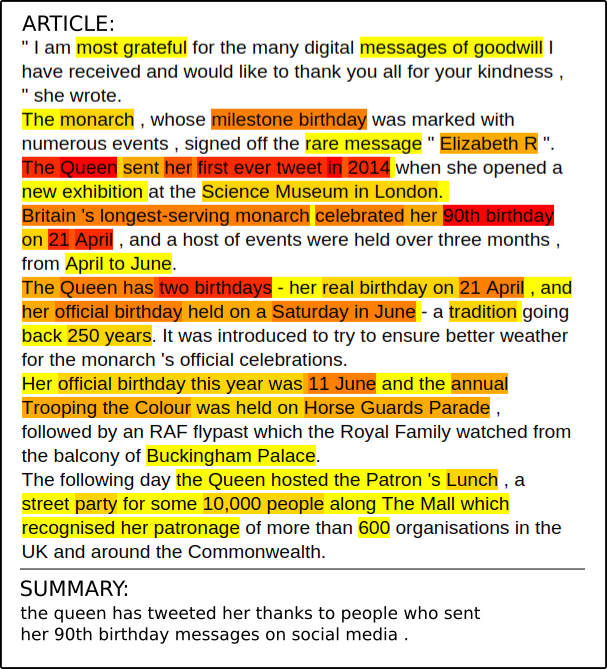
\includegraphics[width=7.6cm]{heatmap_summ}
    \caption{Highlight-based evaluation of summaries. Annotators to evaluate a summary (bottom) against the highlighted source document (top) presented with a heat map marking the salient content in the document; the darker the colour, the more annotators deemed the highlighted text salient. %We describe in Section~\ref{sec:highres} the annotation of document highlights and the evaluation of summaries.
    }
  \label{image:heatmap}
\end{figure}

Measuring progress in summarization is difficult, as the task has as input a source document consisting of multiple sentences and methods need to generate a shorter text that expresses the salient information of the source fluently and succinctly. Thus there can be multiple equally good summaries for the same source document as not all salient information can fit in a given summary length, while even extractive methods that select complete sentences are not guaranteed to produce a coherent summary overall.

The most consistently used evaluation approach is comparison of the summaries produces against reference summaries via 
automatic measures such as ROUGE \citep{Lin2004} and its variants. However, automatic measures are unlikely to be sufficient to measure performance in summarization \citep{schluter:2017:EACLshort}, also known for other tasks in which the goal is to generate natural language \citep{novikova2017we}. Furthermore, the datasets typically considered have a single reference summary, as obtaining multiple ones increases dataset creation cost, thus evaluation against them is likely to exhibit reference bias \citep{Louis2013,fomicheva2016reference}, penalizing summaries containing salient content different from the reference. 

For the above reasons manual evaluation is considered necessary for measuring progress in summarization. However, the intrinsic difficulty of the task has led to research without manual evaluation or only fluency being assessed manually.  Those that conduct manual assessment of the content, typically use a single reference summary, either directly \citep{Celikyilmaz2018, Tan2017} or through questions \citep{narayan18xsum,Narayan2018} and thus are also likely to exhibit reference bias. 
%In addition to that, new metrics are also appearing every year, e.g.\ the ``correctness'' of summary \citep[e.g.][]{Li2018b, Chen2018a}.

%Up to now, too little attention has been paid to build a consensus in manual evaluation framework which has eventually lead to a fragmented field and many unnecessary system evaluation rerun due to non-reusable results. Summarization field used to have a common manual evaluation practice that is established through DUC such as Pyramid method \citep{Nenkova2004} but then the method would need expert annotators for every new dataset which is costly. Furthermore, the method is also prone to reference bias when there is only one summary available for every document.

In this paper we propose a novel approach for manual evaluation, \textsc{High}light-based \textsc{R}eference-less \textsc{E}valuation of document \textsc{S}ummarization (\highres), in which a summary is assessed against the source document via manually highlighted salient content in the latter (see Figure~\ref{image:heatmap} for an example). Our approach avoids reference bias, as the multiple highlights obtained help consider more content than what is contained in a single reference. The highlights are not dependent on the summaries being evaluated but only on the source documents, thus they are reusable across studies, and they can be crowd-sourced more effectively than actual summaries. %In addition to that, we also proposed an automatic weighted n-gram evaluation that is calculated using the highlights and article.
Furthermore, we propose to evaluate the clarity of a summary separately from its fluency, as they are different dimensions.
Finally, \highres\ provides absolute instead of ranked evaluation, thus the assessment of a system can be conducted and interpreted without reference to other systems.

%AV:
%- absolute
% -reference free
% highlights improve the assessment of content
% Previous work does content with the pyramid (we need to redo for every new system summary with experts), factual correctness (ignores saliency), coverage/informativeness (either reference-based or each judge has his/her own reference in mind which leads to inconsistency)


%Highlight-bAsed Evaluation of Single document Summarization (HArnESS) which makes three contributions: 
%(1) We present a new way to assess a content of summary by comparing it against the original document, facilitated through manually highlighted salient document. (2) We provide a complete manual evaluation framework for evaluating the quality of summary that yields reusable result and does not require expert annotators. (3) We provide a new augmented annotation for XSum dataset.  

To validate our proposed approach we use the recently introduced e\textsc{X}treme \textsc{Sum}marization dataset \citep[\xsum,][]{narayan18xsum} to evaluate two state-of-the-art abstractive summarization methods, Pointer Generator Networks \citep{See2017} and Topic-aware Convolutional Networks \citep{narayan18xsum}, using crowd-sourcing for both highlight annotation and quality judgments.
%We ensure the reliability of our results by putting sanity checks (detailed more in Section~\ref{sec:highres}) at the end of our annotation and evaluation tasks.
We demonstrate that \highres{} improves inter-annotator agreement in comparison to using the source document directly, while they help emphasize differences among systems that would be ignored under other evaluation approaches, including reference-based evaluation. Furthermore, we show that the clarity metric from the DUC \citep{dang2005overview} must be measured separately from ``fluency'', as judgments for them had low correlation. %We demonstrate our findings with both quantitative and qualitative analyses.
Finally, we make the highlighted \xsum\ dataset, codebase to replicate the crowd-sourcing experiments and all other materials produced in our study publicly available.


%We have shown that we obtained similar ranking between \ptgen{} and \tconv{} with the automatic and content evaluation results produced by \citet{narayan18xsum}. 

%The remainder of this paper is organized as follows. Section~\ref{tab:litreview} provides a literature review of manual evaluation in recent years. In Section~\ref{sec:highres}, we present our \highres{} framework. Section~\ref{sec:data-models} detail the dataset and models for our framework validation, and Section~\ref{sec:exp-res} discuss the experiment and result. Section~\ref{sec:qanalysis} analyze and exemplify the result quantitatively. Discussion of the future work concludes this paper. 
\begin{table*}[th!]
\centering
\small
\begin{tabular}{r | c c c c c c c | c c | c c r}

\hline
\rotatebox[origin=c]{0}{\textbf{Systems}} &  \rotatebox[origin=l]{90}{\textbf{Pyramid}} & \rotatebox[origin=l]{90}{\textbf{QA}} & \rotatebox[origin=l]{90}{\textbf{Correctness}} &
\rotatebox[origin=l]{90}{\textbf{Fluency}} &
\rotatebox[origin=l]{90}{\textbf{Clarity}} & \rotatebox[origin=l]{90}{\textbf{Recall}} & \rotatebox[origin=l]{90}{\textbf{Precision}} & \rotatebox[origin=l]{90}{\textbf{Absolute}} & \rotatebox[origin=l]{90}{\textbf{Relative}} & \rotatebox[origin=l]{90}{\textbf{With Reference}} & \rotatebox[origin=l]{90}{\textbf{With Document}} & \rotatebox[origin=l]{90}{\textbf{With Ref. \& Doc.}} \\
\hline
% \cite{See2017}        &  $\checkmark$   &   &    &   &  &  &   &    &      &     &    &     &  \\
% \cite{Perrin2017}     &  $\checkmark$   &   &    &   &  &  &   &    &      &     &    &     &  \\
% \cite{Cohan2018a}     &  $\checkmark$   &   &    &   &  &  &   &    &      &     &    &     &  \\
% \cite{Liao2018a}      &  $\checkmark$   &   &    &   &  &  &   &    &      &     &    &     &  \\
% \cite{Kedzie2018}     &  $\checkmark$   &   &    &   &  &  &   &    &      &     &    &     &  \\
% \cite{Amplayo2018a}   &  $\checkmark$   &   &    &   &  &  &   &    &      &     &    &     &  \\
% \cite{Jadhav2018a}    &  $\checkmark$   &   &    &   &  &  &   &    &      &     &    &     &  \\
% \cite{Li2018c}        &  $\checkmark$   &   &    &   &  &  &   &    &      &     &    &     &  \\
% \cite{Pasunuru2018a}  &  $\checkmark$   &   &    &   &  &  &   &    &      &     &    &     &  \\
% \cite{Cao2018a}       &  $\checkmark$   &   &    &   &  &  &   &    &      &     &    &     &  \\
% \cite{Sakaue2018a}    &  $\checkmark$   &   &    &   &  &  &   &    &      &     &    &     & \\
\citet{Celikyilmaz2018}       &  &  &    &  &  &  $\checkmark$ &  $\checkmark$    &  $\checkmark$   &  $\checkmark$     &  $\checkmark$    &  $\checkmark$   & \\
\citet{Chen2018a}     &   &  & $\checkmark$   & & &  $\checkmark$ &  $\checkmark$    &    &  $\checkmark$     &     &    &  $\checkmark$   \\

\citet{Guo2018a}        &   &  &   &  $\checkmark$  & &  &  $\checkmark$    &    &  $\checkmark$     &     &    &  $\checkmark$  \\
\citet{Hardy2018}      &   &  &   & $\checkmark$  & &   &     & $\checkmark$  &      &     &    &   \\
\citet{Hsu2018}         &  &  &    &  $\checkmark$  & &  $\checkmark$ &  $\checkmark$    &  $\checkmark$   &      &     &  $\checkmark$   &  \\
\citet{Krishna2018a}       &   &  &   &  &  &  $\checkmark$ &     &    &  $\checkmark$     &     &  $\checkmark$   &    \\
\citet{Kryscinski2018}     &   &  &   &  $\checkmark$ & &  $\checkmark$ & &  $\checkmark$   &      &  & $\checkmark$ &   \\
\citet{Li2018a}         &   &   & $\checkmark$ &  &  &   &     &  $\checkmark$   &      &     &     &    \\
\citet{narayan-sidenet18}      & &   &    &  $\checkmark$ & &  &     &    & $\checkmark$ &  &  $\checkmark$   &    \\
\citet{narayan18xsum}          &   &  $\checkmark$ &    &  $\checkmark$ &  &  $\checkmark$ &     &  $\checkmark$  &  $\checkmark$     &   $\checkmark$  &  $\checkmark$   &   \\
\citet{Narayan2018}       &   & $\checkmark$ &   &  $\checkmark$  & &  $\checkmark$ &     &  $\checkmark$  &  $\checkmark$   &  $\checkmark$   &  $\checkmark$  &   \\
\citet{Peyrard2018a}     &   &  &   &  &  &  $\checkmark$ &  $\checkmark$    &  $\checkmark$   &      &  $\checkmark$    &    &   \\
\citet{ShafieiBavani2018}      &  $\checkmark$ &  &    &  &  &  &     &    &      &     &    &  \\
\citet{Song2018}       &   &  & $\checkmark$   &  $\checkmark$ &  &  $\checkmark$ &     &  $\checkmark$   &      &     &  $\checkmark$   & \\
\citet{Yang2017b}       &  &  &    &  &  &  $\checkmark$ &     &    &  $\checkmark$     &  $\checkmark$    &    & \\
\highres\ (ours)    &   &  &   & $\checkmark$ & $\checkmark$ & $\checkmark$  &  $\checkmark$   & $\checkmark$  &      &     &  $\checkmark$  &   \\
\hline
\end{tabular}
\caption{Overview of manual evaluations conducted in recent summarization systems. We categorize them in three dimensions: the first column identifies matrices used for evaluating content (``\textit{Pyramid}'', ``\textit{QA}'', ``\textit{Correctness}'', ``\textit{Recall}'' and ``\textit{Precision}'') and quality (``\textit{Clarity}'', ``\textit{Fluency}'') of summaries; the second column focuses if the system ranking reported by humans on content evaluation were ``\textit{Absolute}'' or ``\textit{Relative}''; and finally, the third column evaluates if summaries were evaluated against the input document (``\textit{With Document}''), the reference summary (``\textit{With Reference}'') or both (``\textit{With Ref. \& Doc.}'').}
\label{tab:litreview}
\end{table*}

\section{Literature Review}
\label{sec:review}

In recent years, summarization literature has investigated different means of conducting manual evaluation. We study a sample of 26 recent papers from major ACL conferences and outline the trends of manual evaluation in summarization in Table~\ref{tab:litreview}. From 26 papers, 11 papers \citep[e.g.,][]{See2017,Kedzie2018,Cao2018a} did not conduct any manual evaluation, they are not shown in Table~\ref{tab:litreview}.\footnote{A complete table from this study can be found in the supplementary material.}  Following the Document Understanding Conference (DUC) \citep{dang2005overview}, a majority of work has focused on evaluating the content and the linguistic quality of summaries \cite{Nenkova:2005:ATS}. However, there seems to be a lack of consensus on how a summary should be evaluated: (i) Should it be evaluated relative to other summaries or standalone in absolute terms? and (ii) What would be a good source of comparison: the input document or the reference summary? The disagreements on these issues result in authors evaluating their summaries often (11 out of 26 papers) using automatic measures such as ROUGE \cite{Lin2004} despite of its limitations \cite{schluter:2017:EACLshort}. 
In what follows, we discuss previously proposed %manual evaluation
approaches along three axes: evaluation metrics, relative vs. absolute, and the choice of reference.

\paragraph{Evaluation Metrics}
Despite differences in the exact definitions,
the majority \citep[e.g.,][]{Hsu2018,Celikyilmaz2018,narayan18xsum,Chen2018a,Peyrard2018a} agree on both or either one of two broad quality definitions: {\em coverage} determines how much of the salient content of the source document is captured in the summary,
and {\em informativeness}, 
how much of the content captured in the summary is salient with regards to the original document.
These measures correspond to 
``\textit{recall}'' and ``\textit{precision}'' metrics respectively in Table~\ref{tab:litreview}, notions that are commonly used in information retrieval and information extraction literature.
\citet{Clarke2010} proposed a question-answering based approach to improve the agreement among human evaluations for the quality of summary content, which was recently employed by \citet{narayan18xsum} and \citet{Narayan2018} (QA in Table~\ref{tab:litreview}). In this approach,  questions were created first from the reference summary and then the system summaries were judged with regards to whether they enabled humans to answer those questions correctly. \citet{ShafieiBavani2018}, on the other hand, used the ``Pyramid'' method \citep{Nenkova2004a} which requires summaries to be annotated by experts for salient information. %Nevertheless, the latter two approaches are prone to reference bias \citep{Louis2013}.
A small number of work evaluates the "Correctness" \citep{Chen2018a,Li2018a,Chen2018a} of the summary, similar to fact checking \cite{vlachos-riedel:2014:W14-25}, which can be a challenging task in its own right.

The linguistic quality of a summary encompasses many different qualities such as fluency, grammatically, readability, formatting, naturalness and coherence. Most recent work uses 
a single human judgment
to capture all linguistic qualities of the summary \cite{Hsu2018,Kryscinski2018,narayan18xsum,Song2018,Guo2018a}; we group them under ``Fluency'' in Table~\ref{tab:litreview} with an exception of ``Clarity'' which was evaluated in the DUC evaluation campaigns \citep{dang2005overview}. The ``Clarity'' metric puts emphasis in easy identification of noun and pronoun phrases in the summary which is a different dimension than ``Fluency'', as a summary may be fluent but difficult to be understood due to poor clarity. % \footnote{The ``Clarity'' guidance can be seen in }.

\paragraph{Absolute vs Relative Summary Ranking.} 
In relative assessment of summarization, 
annotators are shown two or more summaries and are asked to rank them according to the dimension at question \citep{Yang2017b,Chen2018a,narayan-sidenet18,Guo2018a,Krishna2018a}. The relative assessment is often done using the paired comparison \citep{Thurstone1994} or the best-worst scaling \citep{Woodworth1991,Louviere2015}, to improve inter-annotator agreement. On the other hand,
absolute assessment of summarization \cite{Li2018a,Song2018,Kryscinski2018,Hsu2018,Hardy2018} 
is often done using the Likert rating scale \citep{Likert1932} where a summary is assessed on a numerical scale. 
Absolute assessment was also employed in combination with the question answering approach for content evaluation
\citep{narayan18xsum,Narayan2018}. Both approaches, relative ranking and absolute assessment, have been investigated extensively in Machine Translation \citep{Bojar2016, Bojar2017}. %It has been shown that the 
 Absolute assessment correlates highly with the relative assessment without the bias introduced by having a simultaneous assessment of several models \citep{Bojar2011}. %In our study we use the direct assessment of summaries using the  Likert rating scale (1-100).

\paragraph{Choice of Reference.} 
The most convenient
way to evaluate a system summary is to assess it against the reference summary \citep{Celikyilmaz2018,Yang2017b,Peyrard2018a}, as this typically requires less effort than reading the source document. The question answering approach of \citet{narayan18xsum,Narayan2018} also falls in this category, as the questions were written using the reference summary. However, summarization datasets are limited to a single reference summary per document \citep{Sandhaus2008,Hermann2015,newsroom_N181065,narayan18xsum} thus evaluations using them
%assessing a summary against a single reference summary
is prone to reference bias \citep{Louis2013}, also a known issue in machine translation evaluation \citep{fomicheva2016reference}. A circumvention for this issue is to evaluate it against the source document \citep{Song2018,narayan-sidenet18,Hsu2018,Kryscinski2018}, asking judges to assess the summary after reading the source document. However this requires more effort and is known to lead to low inter-annotator agreement \citep{Nenkova2004a}. 




% Previous work does content with the pyramid (we need to redo for every new system summary with experts), factual correctness (ignores saliency), coverage/informativeness (either reference-based or each judge has his/her own reference in mind which leads to inconsistency)


%Highlight-bAsed Evaluation of Single document Summarization (HArnESS) which makes three contributions: 
%(1) We present a new way to assess a content of summary by comparing it against the original document, facilitated through manually highlighted salient document. (2) We provide a complete manual evaluation framework for evaluating the quality of summary that yields reusable result and does not require expert annotators. (3) We provide a new augmented annotation for XSum dataset.  


% % % Hardy
% A large and growing body of summarization literature has investigated different means of doing manual evaluation. We have look into a sample of 24 recent papers (see Appendix) from major conference to see the trends of manual evaluation and discovered that 10 papers didn't perform manual evaluation at all, while only 5 papers performed a complete content and linguistic quality evaluations. Most papers either focusing on linguistic quality or on the content evaluation. There are also a variety of methods and different metrics' definition used in doing manual evaluation.  In this section, we highlight several of the most prominent ones in terms of metrics and methods.

% \subsection{Evaluation Metrics}
% The Document Understanding Conference (DUC)\footnote{The online proceedings of the conferences are available at \url{http://duc.nist.gov/}} has defined the quality of summary on two broad categories: the content and linguistic of the summary. We will look into recent trend in summarization researches in evaluating these two categories.

% \paragraph{Summary Content Evaluation} The content of summary encompasses many different qualities such as informativeness, coverage, coherence, correctness and etc. Due to the large number of possible quality, there has been little agreement on how to evaluate the quality of summary content. However, we notice that overall, the majority (e.g.: \citep{Hsu2018, Celikyilmaz2018, narayan18xsum, Chen2018a} agree on both or either one of two broad quality definitions: coverage which determine how well does the summary capture the important parts of the article, and informativeness which determine how concise is information in the summary. These qualities correlate to recall and precision metrics that are commonly used in information retrieval and automatic summarization literature. A small number of literature introduces the correctness quality \citep{Chen2018a, Li2018b} which is similar to fact verification. This study follows the majority defined content qualities: coverage and informativeness. 

% \paragraph{Linguistic Evaluation} The linguistic evaluation also encompasses many different qualities such as fluency, grammatically, readability, formatting, naturalness and etc. Most of the researches (e.g.: \citep{Hsu2018, Kryscinski2018, narayan18xsum}) use just one broad category to capture all linguistic qualities of the summary. This research follows the current practice to use just one quality standard to capture the linguistic qualities. We also added the clarity quality which defined as the how much difficulties in identifying the referents of the noun phrases or understanding the meaning of the sentence. The clarity of the quality is first defined in the DUC but hasn't been used by recent researches.

% \subsection{Evaluation Methods}
% Recent advances in evaluating the summary can be broadly categorized into intrinsic and extrinsic evaluations. The intrinsic evaluation which is the majority assess the quality of the summary directly by comparing with the reference or the salient part of the article, while the extrinsic evaluation assess use other approach such as question answering (QA) \citep{Clarke2010, narayan18xsum, Narayan2018}. This study focus on the intrinsic evaluation since it doesn't need any intermediary step such as building questions for QA to assess the summary which requires an expert. 

% Most researches in the intrinsic evaluation mostly differ on two aspects: the object of comparison, and summary scoring. 

% \paragraph{Object of Comparison} On the object of comparison, there are two distinct ways: using predefined references or let the judge to define its own references by reading the article. Using predefined references are normally done by either using the reference summaries directly or asking experts to annotate salient information from the article (e.g.: Pyramid method \citep{Nenkova2004}). Nevertheless, these approaches are prone to reference bias \citep{Louis2013} or low inter-annotator agreements \citep{Nenkova2004}. In a newer released dataset (e.g.: CNN/Daily Mail and XSum) where only single summary is available with no expert annotation, asking the judges to form its own reference by reading the article directly is a norm. These approach however, is not ideal and would yield a high variability between judges' score especially when facing an article that have multiple viewpoints.   

% \paragraph{Summary Scoring} There are two approaches for scoring a summary: relative ranking (RR) assessment (e.g.: \citet{Fan2018, Celikyilmaz2018, narayan18xsum}) or direct assessment (DA) (e.g.: \citet{Kryscinski2018}). A relative ranking assessment can use paired comparison \citep{Thurstone1994} or best-worst scaling \citep{Woodworth1991}, while an direct assessment usually use rating scale \citep{Likert1932}. The usage of relative ranking and direct assessment has been investigated in Machine Translation (MT) field \citep{Bojar2016, Bojar2017} of which it has been shown that DA assessment correlate highly with RR assessment without the bias introduced by having a simultaneous assessment of several models \citep{Bojar2011}. Since the result is an absolute score, it is also reusable for subsequent researches. For this research we use the DA approach from MT with analogue score between 1-100. 

\section{\highres}
\label{sec:highres}

%AV: Moved here from the literature review

Our novel highlight-based reference-less evaluation does not suffer from reference bias as a summary is assessed against the source document with manually highlighted salient content. These highlights are crowd-sourced effectively without the need of expert annotators as required by the Pyramid method \citep{Nenkova2004a} or to generate reference summaries. Our approach improves over the ``Correctness'' or ``Fluency'' only measure for summarization by taking salience into account. Finally, the assessment of summaries against the document with  highlighted pertinent content facilitates an absolute evaluation of summaries with high inter-annotator agreement. 

Our evaluation framework comprises three main components: document highlight annotation, highlight-based content evaluation, and 
clarity and fluency evaluation. The second component, which evaluates the notions of ``Precision'' and ``Recall'' requires the highlights from the first one to be conducted. However, the highlight annotation needs to happen only once per document, and it can be reused to evaluate many system summaries, unlike the Pyramid approach \citep{Nenkova2004a} that requires additional expert annotation for every system summary being evaluated. The third component is independent of the others and can be run in isolation. In all components we employ crowd-workers as human judges, and implement appropriate sanity checking mechanisms to ensure good quality judgements. Finally, we present an extended version of ROUGE \cite{Lin2004} that utilizes the highlights to evaluate system summaries against the document; this demonstrates another use of the highlights for summarization evaluation. 

% Our evaluation framework comprises three components: highlight annotation, highlight-based evaluation, and 
% clarity and fluency evaluation. The second component, which evaluates the notions of ``Precision'' and ``Recall'' requires the highlights from the first one to be conducted. However, the highlight annotation needs to happen only once per document, and it can be reused to evaluate many system summaries, unlike the Pyramid approach \citep{Nenkova2004} that requires additional expert annotation for every system summary being evaluated. The third component is independent of the others and can be run in isolation. %No expert annotation is required in all parts.
% In all components we employ crowdworkers as human judges, and implement appropriate sanity checking mechanisms to ensure good quality judgements.


\subsection{Highlight Annotation}
\label{subsec:hannot}
In this part, we ask human judges to read the source document and then highlight words or phrases that are considered salient. %as important for the article. 
Each judge is allowed to highlight parts of the text at any granularity, from single words to complete sentences or even paragraphs. However we enforce a limit in the number of words to $\mathcal{K}$ that can be highlighted in total by a judge in a document, corresponding to the length of the summary expected.
%To help the judges decide which part of the article should be highlighted we give domain specific guidance. In our experiment using a newswire dataset, we guide the judges using 5W1H (Who, What, When, Where, Why and How) principles \citep{Robertson1946} that is a common practice in journalism. The judges however are not obliged to fulfill all of the guidance content and are instead limited to a maximum of 30 words highlight. 
By employing multiple judges per document who are restricted in the amount of text that can be highlighted  we expect to have a more diverse and focused highlight from multiple judges which cover different viewpoints of the article.

To ensure that each highlight is reliable, we performed a sanity check at the end of the task where we ask the judges to answer a True/False question based on the article. We rejected all annotations that failed to correctly answer the sanity check question. 

%All highlight results are stored in json format to be used in later stage. 

\subsection{Highlight-based Content Evaluation}
In this component, we present human judges a document that has been highlighted using heatmap coloring and a summary to assess (see Figure~\ref{image:heatmap} for an example). We ask our judges to assess the summary for (i) \textit{`All important information is present in the summary'} and (ii) \textit{`Only important information is in the summary.'} The first one is the recall (content coverage) measure and the second, the precision (informativeness) measure. All the ratings were collected on a 1-100 Likert scale \citep{Likert1932}. Figure~\ref{image:highlightbasedevaluation} shows the screen that is presented to judges where salient parts of the document are highlighted.

\begin{figure*}[h]
    \centering
    \fbox{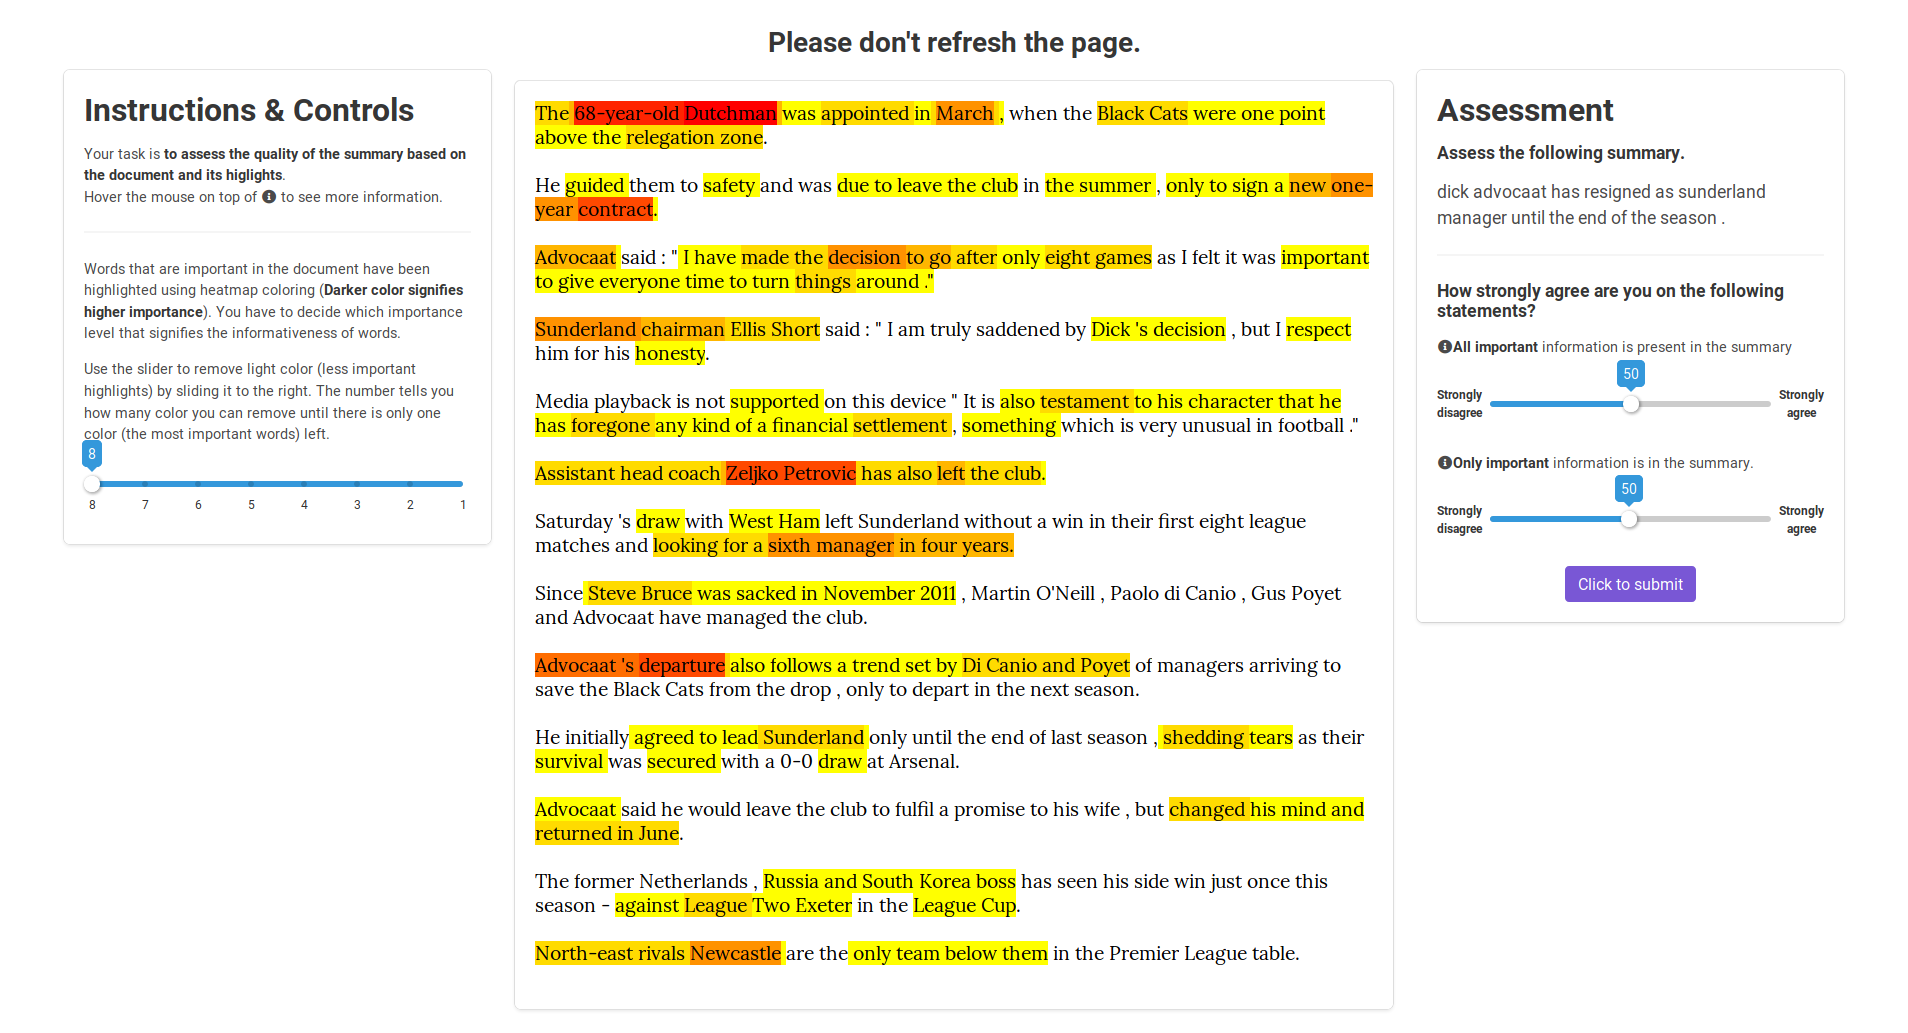
\includegraphics[width=15.5cm]{highlight_evaluation}}
    \label{image:highlightbasedevaluation}
    \caption{The UI for content evaluation with highlight. Judges are given an article with important words highlighted using heat map. Judges can also remove less important highlight color by sliding the scroller at the left of the page. At the right of the page judges give the recall and precision assessment by sliding the scroller from 1 to 100 based on the given summary quality.}
\end{figure*}

As with the highlight annotation, %to ensure that each rating is reliable, 
we performed the same form of sanity check to the one in the highlight annotation task.


\subsection{Clarity and Fluency Evaluation}
In this part, we give the judges only the summary and ask them to rate it on clarity and fluency. For {\em clarity}, each judge is asked whether the summary is easy to be understood, i.e.\ 
there should be no difficulties in identifying the referents of the noun phrases (every noun/place/event should be well-specified) or understanding the meaning of the sentence. For {\em fluency}, each judge is asked whether the summary sounds natural and has no grammatical problems. % that makes the text difficult to read.
While fluency is often evaluated in recent work, clarity, while first introduced in DUC evaluations, has recently been ignored in manual evaluation, despite that it captures a different dimension of summarization quality.

To ensure that the judgments for clarity and fluency are not affected by each other (poor fluency can affect clarity, but a summary can have perfect fluency but low clarity), % is no bias between clarity and fluency evaluation,
we evaluate each metric separately. We ask the judges to evaluate multiple summaries per task with each dimension in its own screen. For sanity checking, we insert three fake summary with different qualities (good, mediocre and bad summaries). We reject results where the numeric scores given by annotators failed to pass this criteria: bad $<$ mediocre $<$ good.

\subsection{Highlight-based ROUGE Evaluation} 
\label{subsec:hrouge}

%ROUGE \cite{Lin2004} %in its traditional setting is used to evaluate system summaries against reference summaries. We extend it to directly evaluate system summaries against the highlighted documents, which implicitly contain multiple summaries as the highlights are obtained from multiple workers. 

Our Highlight-based \rouge{} (we refer to it as \hrouge{}) formulation is similar to the original ROUGE with the difference that the n-grams are weighted by the number of times they were highlighted. One benefit of \hrouge{} is that it introduces saliency into the calculation without being reference-based as in \rouge{}. Implicitly \hrouge{} considers multiple summaries as the highlights are obtained from multiple workers. 

Given a document $\mathcal{D}$ as a sequence of $m$ tokens $\{w_1, \ldots, w_m\}$, annotated with $\mathcal{N}$ highlights, we define the weight $\beta_g^n \in [0,1]$ for an $n$-gram $g$ as: 
\begin{equation}
    \beta_g^n = \frac{\displaystyle\sum_{i=1}^{m-(n-1)} \Bigg[\frac{\sum_{j=i}^{i+n-1} \frac{\mathrm{NumH}(w_j)}{\mathcal{N}}}{n}\Bigg]_{w_{i:i+n-1} == g}}{\displaystyle\sum_{i=1}^{m-(n-1)} [1]_{w_{i:i+n-1} == g} }
\end{equation}
\noindent where, $[x]_y$ is an indicator function which returns $x$ if $y$ is true and $0$, otherwise.  $\mathrm{NumH}(w_j) = \sum_{k=1}^{\mathcal{N}} \frac{\mathrm{len}(H_k)}{\mathcal{K}} [1]_{w_j \in H_k}$ is a function which returns the number of times word $w_j$ is highlighted by the annotators out of $\mathcal{N}$ times weighted by the lengths of their highlights; $H_k$ is the highlighted text by the $k$th annotator and  $\mathcal{K}$ is the maximum allowed length of the highlighted text (see Section~\ref{subsec:hannot}). $\mathrm{NumH}(w_j)$ gives less importance to  annotators with highlights with few words. In principle, if an $n$-gram is highlighted by every crowd-worker and the length of the highlight of each crowd-worker is $\mathcal{K}$, the $n$-gram $g$ will have a maximum weight of $\beta_g^n = 1$.
% \begin{equation}
%     \operatorname{NumH}(w_j) = \displaystyle\sum_{k=1}^{\mathcal{N}} \frac{\operatorname{lenH_k}}{\mathrm{maxLen}} 1_{H_k(w_j)}
% \end{equation}
% \noindent where $1_{H_k(w_j)}$ is an indicator function whether a word $w_j$ is part of the highlight set, $H_k$, $\mathrm{maxLen}$ is the maximum allowed highlight length, % that is set as 30 in our experiment, 
% and $\operatorname{lenH_k}$ is the length of the highlight, $H_k$. 
% The weight for each $n$-gram is estimated using the highlights of each word within it for simplicity.
The HROUGE scores for a summary $\mathcal{S}$ can then be defined as:
\begin{align}
    \text{HR}_{\mathrm{rec}}^n &= \frac{\displaystyle\sum_{g \in n\operatorname{-gram}(\mathcal{S})} \beta_g^n\, \text{count}(g, \mathcal{D} \cap \mathcal{S})}{\displaystyle\sum_{g \in n\operatorname{-gram}(\mathcal{D})} \beta_g^n\,\text{count}(g, \mathcal{D})} \\
    \text{HR}_{\mathrm{pre}}^n &= \frac{\displaystyle\sum_{g \in n\operatorname{-gram}(\mathcal{S})} \beta_g^n\, \text{count}(g, \mathcal{D} \cap \mathcal{S})}{\displaystyle\sum_{g \in n\operatorname{-gram}(\mathcal{S})} \text{count}(g, \mathcal{S})}
\end{align}
\noindent $\text{HR}_{\mathrm{rec}}^n$ and $\text{HR}_{\mathrm{pre}}^n$ are the HROUGE recall and precision scores; $\text{count}(g, \mathcal{X})$ is the maximum number of $n$-gram $g$ occurring in the text $\mathcal{X}$. The weight in the denominator of $\text{HR}_{\mathrm{pre}}^n$ is uniform ($\beta^n_g = 1$) for all $g$ because if we weighted according to the highlights, words in the summary that are not highlighted in the original document would be ignored. This would result in $\text{HR}_{\mathrm{pre}}^n$ not penalizing summaries for containing words that are likely to be irrelevant as they do not appear in the highlights of the document.
%, any addition of junk words to the summary that doesn't appear in the highlight doesn't reduce the final precision. However, this would also limits the maximum precision to lower than 1 when there are multiple highlight annotations.
It is important to note \hrouge{} has an important limitation in that it penalizes abstractive summaries that do not reuse words from the original document. This is similar to \rouge{} penalizing summaries for not reusing words from the reference summaries, however the highlights allow us to implicitly consider multiple references without having to actually obtain them.  %produced with lower annotation effort.

\section{Summarization Dataset and Models}
\label{sec:data-models}

We use the extreme summarization dataset \citep[\xsum,][]{narayan18xsum}\footnote{\url{https://github.com/EdinburghNLP/XSum}} which comprises BBC articles paired with their single-sentence summaries, provided by the journalists writing the articles. The summary in the \xsum\ dataset demonstrates a larger number of novel $n$-grams compared to other popular datasets such as CNN/DailyMail \citep{Hermann2015} or NY Times \citep{Sandhaus2008} as such it is suitable to be used for our experiment since the more abstractive nature of the summary renders automatic methods such as ROUGE less accurate as they rely on string matching, and thus calls for human evaluation for more accurate system comparisons. 
% This makes the dataset suitable for our experiment since we do not want the judges to be biased towards extractive methods which makes the process of assessment easier compared to the abstractive methods. In other words, we expect in an abstractive setting, the task of reading an article will be more laborious and prone to disagreement between judges.
Following \citet{narayan18xsum}, we didn't use the whole test set portion, but sampled 50 articles from it for our highlight-based evaluation.  

% We didn't use the whole test set portion for evaluation, but sampled 50 articles from it for our experiments with human evaluation, following \citet{narayan18xsum}.

We assessed summaries from two state-of-the-art abstractive summarization systems using our highlight-based evaluation: (i) the Pointer-Generator model (\ptgen) introduced by \citet{See2017} is an RNN-based abstractive systems which allows to copy words from the source text, and (ii) the Topic-aware Convolutional Sequence to Sequence model (\tconv) introduced by \citet{narayan18xsum} is an   abstractive model which is conditioned on the article's topics and based entirely on Convolutional Neural Networks.
We used the pre-trained models\footnote{Both models were trained using the standard cross-entropy loss to maximize the likelihood of the reference summary given the document.} provided by the authors to obtain summaries from both systems for the documents in our test set.

% \footnote{\url{https://github.com/abisee/pointer-generator}} \citep{See2017}.

\section{Experiments and Results}
\label{sec:exp-res}

All of our experiments are done using the Amazon Mechanical Turk platform. %We use our newly proposed \highres\ to evaluate \ptgen\ and \tconv\ on \xsum. 
We develop three types of Human Intelligence Tasks (HITs): highlight annotation, highlight-based content evaluation, and fluency and clarity evaluation. In addition, we elicited human
judgments for content evaluation in two more ways: we assessed system summaries against the original document (without highlights) and against the reference summary. 
% We also run two more types of content evaluation using the same questions for precision and recall: one against the source document (without highlights) and one against the reference. 
The latter two experiments are intended as the comparison for our proposed highlight-based content evaluation.

\subsection{Highlight Annotation} 

We collected highlight annotations from 10 different participants for each of 50 articles. For each annotation, we set  $\mathcal{K}$, the maximum number of words to highlight, to 30. Our choice reflects the average length (24 words) of reference summaries in the \xsum\ dataset. To facilitate the annotation of BBC news articles with highlights, we asked our participants to adapt the 5W1H (Who, What, When, Where, Why and How) principle \citep{Robertson1946} that is a common practice in journalism. The participants however were not obliged to follow this principle and were free to highlight content as they deem fit. 

% For the highlight annotation, we run the annotation 10 times for each of the 50 articles. For each task, we limit the annotation process to 10 minutes and 30 words maximum, since the intended summary in \xsum\   is a single sentence. 

% \begin{figure*}[t!]
%     \centering
%     \begin{minipage}{.45\textwidth}
%     \centering
%     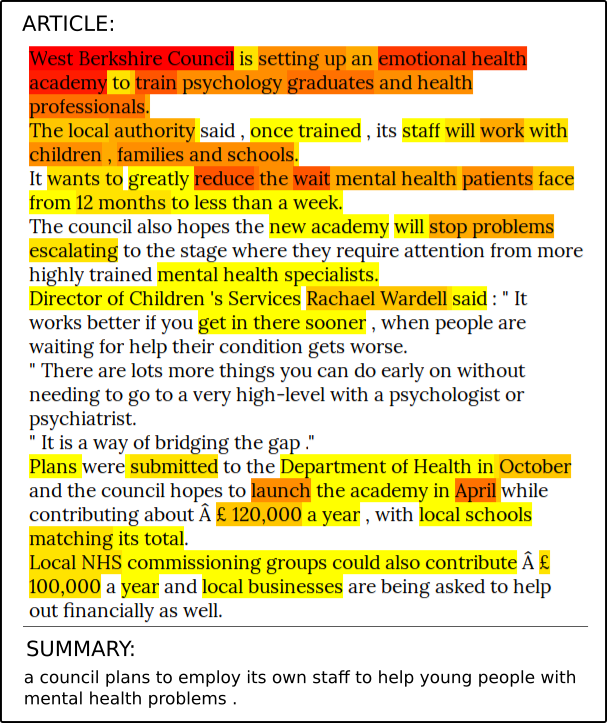
\includegraphics[height=8cm]{heatmap_best}
%     \end{minipage}
%     \begin{minipage}{.45\textwidth}
%     \centering
%     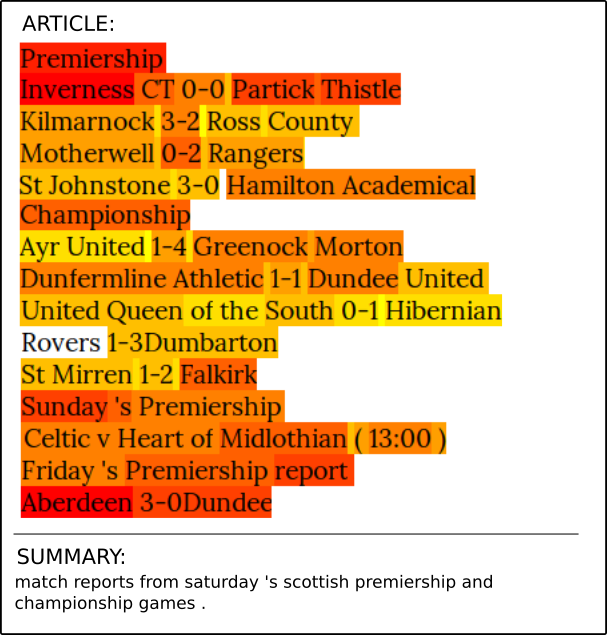
\includegraphics[height=7cm]{heatmap_negative}
%     \end{minipage}
%     \caption{Highlight annotation for the documents with the highest (left) and lowest (right) agreement. We also show their reference summaries at the bottom.}
%   \label{image:heatmap_both}
% \end{figure*}

The resulting annotation exhibits a substantial amount of variance, confirming the intuition that different participants are not expected to agree entirely on what is salient in a document. 
On average, the union of the highlights from 10 annotators covered 38.21\% per article and  33.77\% of the highlights occurred at the second half of the article. This shows that the judges did not focus only on the beginning of the documents but annotated all across the document.

% as we filter out judges that did not read the whole article through sanity checking.

Using Fleiss Kappa \citep{Josep1971} on the binary labels provided by each judge on each word (highlighted or not) we obtained an average agreement of 0.19 for the 50 articles considered. The low agreement score does not indicate a poor annotation process necessarily; we argue that this is primarily due to the annotators having different opinions on which parts of an article are salient. The article with the highest agreement (0.32) has more focused highlights, whereas the article with the lowest agreement (0.04) has highlights spread all over (both articles can be seen in the supplementary materials). Interestingly, the reference summary on the highest agreement article appears to be more informative of its content when the annotator agreement is high; the reference summary on the lowest agreement article is more indicative, i.e., it doesn’t contain any informative content from the article but only to inform the reader about the article’s topic and scope. These results confirms that the annotation behaviour originates from the nature of the document and the summary it requires, and validates our highlight annotation setup.

% Figure~\ref{image:heatmap_both} shows the document (left) with the highest agreement of 0.32 and the document (right) with the lowest agreement is 0.04. As can be seen, the document with a high agreement tends to have more focused highlights, wheres the document with a low agreement has highlights spread all over. The document on the right in Figure~\ref{image:heatmap_both} simply presents a match report from Premiership and Championship games, it is hard for annotators to agree on which game to highlight. Interestingly, the reference summary on the left appears to be more informative of its content for which the annotator agreement is high; the reference summary on the right is more indicative, i.e., it describes the document rather than directly presenting the information it contains. These results confirms that the annotation behaviour originates from the nature of the document and the summary it requires, and validates our highlight annotation setup.

% The highest agreement is 0.32 while the lowest agreement is 0.04. 

% The article with the lowest agreement score is the negative sample that we used which heat map can be seen in. 



% We also measure the mean recall, precision and F$_1$ of unigram and bigram between summary and highlight of the reference, \tconv\  and \ptgen\   models as shown in Table \ref{table:overlapsummaryhighlight}.

% \begin{table}[t!]
% % \small
% \centering
% \begin{tabular}{l | p{0.5cm} p{0.5cm} p{0.5cm} | p{0.5cm} p{0.5cm} p{0.5cm}}
% \hline
% \multirow{2}{*}{\textbf{Model }} & \multicolumn{3}{c}{\textbf{Unigram}} & \multicolumn{3}{c}{\textbf{Bigram}}  \\
%                         & Prec  & Rec   & F$_1$        & Prec  & Rec  & F$_1$         \\
% \hline
% \tconv\                 & 79.57 & 4.38 & 8.13 & 28.47 & 1.32 & 2.49         \\
% \ptgen\                     & \textbf{79.94} & \textbf{1.82} & \textbf{9.64}       & \textbf{31.58} & \textbf{1.82} & \textbf{3.39}         \\
% Reference               & 72.74 & 7.82 & 13.90       & 22.43 & 1.31 & 2.46 \\
% \hline
% \end{tabular}
% \caption{The ROUGE score between the document and summary for all models and reference. \todo{merge with table 5, improve caption}}
% \label{table:overlapsummarydocument}
% \end{table}
% Please add the following required packages to your document preamble:
% \usepackage{multirow}
% Please add the following required packages to your document preamble:
% \usepackage{multirow}
\begin{table}[ht!]
\small
\begin{tabular}{l|p{0.4cm}p{0.6cm}|p{0.4cm}p{0.4cm}|p{0.4cm}p{0.4cm}}
\hline
\multirow{3}{*}{\textbf{Model}}                & \multicolumn{2}{c|}{\textbf{Highlight}}                              & \multicolumn{2}{c|}{\textbf{Non High-}} & 
\multicolumn{2}{c}{\textbf{Reference}}\\
\multirow{2}{*}{}                
& \multicolumn{2}{c|}{\textbf{-based}}                              & \multicolumn{2}{c|}{\textbf{light-based}} & 
\multicolumn{2}{c}{\textbf{-based}}\\
& \textbf{Prec} & \textbf{Rec} 
& \textbf{Prec} & \textbf{Rec}
& \textbf{Prec} & \textbf{Rec} \\ \hline
\tconv{} & 57.42 & 49.95 & 52.55 & 41.04 & 46.75 & 36.45             \\
\ptgen{} & 50.94 & 44.41 & 48.57 & 39.21  & 44.24 & 38.24             \\
Reference & 67.90 & 56.83 & 66.01 & 52.45  & --- & --- \\
\hline
\end{tabular}
\caption{Results of content evaluation of summaries against documents with highlights, documents without highlights and reference summaries.}
\label{table:summresult}
\end{table}

% Please add the following required packages to your document preamble:
% \usepackage{multirow}
\begin{table}[ht!]
\small
\begin{tabular}{l|cc|cc}
\hline
\multirow{2}{*}{\textbf{Model}} & 
\multicolumn{2}{c|}{\textbf{Highlight-based}} & 
\multicolumn{2}{c}{\textbf{Non Highlight-based}} \\
&\textbf{Prec} & \textbf{Rec} & 
 \textbf{Prec} & \textbf{Rec} \\ \hline
\tconv{} & 0.67 & 0.80 & 0.75                             & 0.83  \\
\ptgen{} & 0.73 & 0.86 & 0.73   & 0.90  \\
Reference                             & 0.49                           & 0.63 & 0.48   & 0.67 \\
\hline

\end{tabular}
\caption{Coefficient of variation (lower is better) for evaluating summaries against documents with and without highlights.}
\label{table:summresultcv}
\end{table}
% \begin{table*}[t!]
% \small
% \centering
% \begin{tabular}{l | l | ccc | ccc | ccr }

% \hline

% \multirow{2}{*}{\textbf{Model}}     &      & \multicolumn{3}{c|}{\textbf{Highlight-based}} & \multicolumn{3}{c|}{\textbf{Non Highlight-based}} & \multicolumn{3}{c}{\textbf{Reference-based}} \\
%                           &      & Prec       & Rec        & F$_1$        & Prec        & Rec         & F$_1$          & Prec       & Rec       & F$_1$        \\
% \hline
% \multirow{2}{*}{\tconv\ } & Mean & \textbf{57.42}      & \textbf{49.95}      & \textbf{47.00}     & 52.55       & 41.04       & 39.25       & 46.75      & 36.45     & 36.83     \\
%                           & $cv$   & \textbf{0.67}       & \textbf{0.80}       & \textbf{0.71}      & 0.75        & 0.83        & 0.81        & 0.78       & 0.90      & 0.85      \\
% \multirow{2}{*}{\ptgen\  }     & Mean & \textbf{50.94}      & \textbf{44.41}      & \textbf{42.17}     & 48.57       & 39.21       & 37.80       & 44.24      & 38.24     & 35.83     \\
%                           & $cv$   & \textbf{0.73}       & 0.86       & \textbf{0.81}      & \textbf{0.73}        & 0.90        & 0.84        & 0.78       & \textbf{0.84}      & 0.82      \\
% \multirow{2}{*}{Reference} & Mean & \textbf{67.90}      & \textbf{56.83}      & \textbf{55.25}     & 66.01       & 52.45       & 50.67       & ---        & ---       & ---       \\
%                           & $cv$   & 0.49       & \textbf{0.63}       & \textbf{0.61}      & \textbf{0.48}        & 0.67        & \textbf{0.61}        & ---        & ---       & ---\\
% \hline
% \end{tabular}
% \caption{Results of content evaluation of summaries against documents with highlights (Highlight-based), original documents without highlights (Non Highlight-based) and reference summaries (Reference-based). We evaluate summaries from \tconv and \ptgen\, and the reference summaries. We report on the mean and unbiased coefficient of variation ($cv$, lower values are better) for precision, recall and F$_1$ scores.}
% \label{table:summresult}
% \end{table*}


\subsection{Content Evaluation of Summaries} 
\label{subsec:conteval}

We assessed the %abstractive 
summaries against (i) documents with highlights (Highlight-based), (ii) original documents without highlights (Non Highlight-based) and (iii) reference summaries (Reference-based). For each setup, we collected judgments from 3 different participants for each model summary. Table \ref{table:summresult} and \ref{table:summresultcv} presents our results.

% We experimented with three settings for content evaluation: source document with highlights, source document without highlights and reference-based.
% %The content evaluation consists of the previously mentioned four experiments.
% %The unguided evaluation has all the same settings with the guided one except that there are no highlights in the article. In the reference-only evaluation, we gave the Turkers a single summary reference and a random model summary. 
% Each model summary was evaluated in each setting three times, whose results were averaged after removing those that failed the sanity check.
% %For each model's summary, we run the evaluation three times. 
% Each run asked the crowd-worker to score the informativeness and the coverage of the summary using 1-100 rating. 
% %Since these two scores correlate to recall and precision scores,
% We also calculate the F$_1$ score from them. %We use the term recall and precision interchangeably with coverage and informativeness in this study.

Both the highlight-based and non-highlight based assessment of summaries agree on the ranking among \tconv, \ptgen\ and Reference. Perhaps unsurprisingly human-authored summaries were considered best, whereas, \tconv\ was ranked 2nd, followed by \ptgen. However, the performance difference in \tconv\ and \ptgen\ is greatly amplified when they are evaluated against document with highlights (6.48 and 5.54 Precision and Recall points) compared to when evaluated against the original documents (3.98 and 1.83 Precision and Recall points). The performance difference is lowest when they are evaluated against the reference summary (2.51 and -1.79 Precision and Recall points). The superiority of \tconv\ is expected; \tconv\ is better than \ptgen\ for recognizing pertinent content and generating informative summaries due to its ability to represent high-level document knowledge in terms of topics and long-range dependencies \citep{narayan18xsum}.

% between the two systems is greater in the highlight-based evaluation (5 F$_1$ points) and the smallest for the reference-based one, mostly due to higher recall judgments for \tconv\ , while the reference-based evaluation judges the systems to be equal. The superiority of \tconv\  is expected, as \todo{Shashi, could you add something here?}

%\tconv\  has F$_1$ point higher compared to the \ptgen\   in all experiment settings. Interestingly, in the guided experiment, the mean F$_1$ is 7.75 and 10.17 points higher over the unguided. 

We further measured the agreement among the judges using the coefficient of variation \citep{everitt2006cambridge} from the aggregated results. It is defined as the ratio between the sample standard deviation and sample mean. It is a scale-free metric, i.e.\ its results are comparable across measurements of different magnitude.
%Using the $cv$ score we can compare the variability of different models. The following is the $cv$ equation.
%It is defined as:
%\begin{equation}
%  cv = \frac{\sigma}{\bar{x}}
%\end{equation}
Since, our sample size is  small (3 judgements per summary), we  use the unbiased version \citep{sokal1995biometry} as $cv = (1 + \frac{1}{4n})\frac{\sigma}{\bar{x}}$, where $\sigma$ is the standard deviation, $n$ is the number of sample, and $\bar{x}$ is the mean.

We found that the highlight-based assessment in general has lower variation among judges than the non-highlight based or reference-based assessment. The assessment of \tconv\ summaries achieves 0.67 and 0.80 of Precision and Recall $cv$ points which are 0.08 and 0.03 points below when they are assessed against documents with no highlights, respectively. We see a similar pattern in Recall on the assessment of \ptgen\ summaries. Our results demonstrate that the highlight-based assessment of abstractive systems improve agreement among judges compared to when they are assessed against the documents without highlights or the reference summaries. The assessment of human-authored summaries does not seem to follow this trend, we report a mixed results (0.49 vs 0.48 for precision and 0.63 vs 0.67 for recall) when they are evaluated with and without the highlights.

% has 0.1 and 0.14 $cv$ points lower than the non highlight-based. We also noticed that the improvement of the mean and $cv$ in recall is higher than precision across all models which shows that our highlight approach helps the judges when looking for salient information in the article. Overall we conclude that our highlight-based evaluation has lower variation while improving the score of the models.


\begin{table}[t!]
\small
\centering
\begin{tabular}{l | cr}
\hline
\textbf{Model} & \textbf{Fluency} & \textbf{Clarity} \\
\hline
\tconv\  & 69.51        & 67.19        \\
\ptgen\      & 55.24        & 52.49        \\
Reference      & 77.03        & 75.83       \\
\hline
\end{tabular}
\caption{Mean "Fluency" and "Clarity" scores for \tconv\ , \ptgen\   and Reference summaries. All the ratings were collected on a 1-100 Likert scale.}
\label{table:fluencyclarityresult}
\end{table}

\subsection{Clarity and Fluency Evaluation} 

% In this component we run evaluations for clarity and fluency separately, in order to assess if indeed they evaluate different qualities in the summaries. %In each evaluation, the Turkers have to rate at most 8 random summaries. 

Table \ref{table:fluencyclarityresult} shows the results of our 
fluency and clarity evaluations. Similar to our highlight-based content evaluation, human-authored summaries were considered best, whereas \tconv\  was  ranked  2nd  followed  by  \ptgen, on both measures. 
% As in the case of the content evaluation, the reference summaries are judged superior to both systems. Among the latter, \tconv\  is judged superior, which is expected as it was developed in the context of the \xsum\   dataset. \todo{Shashi, can we say something better?}
The Pearson correlation between fluency and clarity evaluation is 0.68 which shows a weak correlation; it confirms our hypothesis that the "clarity" captures different aspects from "fluency" and they should not be combined as it is commonly done. 

\begin{table}[t!]
\centering
\small
\begin{tabular}{l|cc|cc}
\hline
\multirow{2}{*}{\textbf{Model}} & \multicolumn{2}{c|}{\textbf{Unigram}} & \multicolumn{2}{c}{\textbf{Bigram}} \\
& Prec     & Rec  & Prec     & Rec     \\
\hline 
\multicolumn{5}{c}{\rouge\ (Original document)} \\
\hline
\tconv{}              & \textbf{77.17}    & 4.20    & 26.12    & 1.21    \\
\ptgen{}                  & 77.09    & \textbf{4.99}       & \textbf{28.75}    & \textbf{1.64}      \\
Reference              & 73.65    & 4.42    & 22.42    & 1.17      \\
\hline
\multicolumn{5}{c}{\hrouge\ (Highlights from the document)} \\
\hline
\tconv{}               &   \textbf{7.94}  &  5.42  & 3.30 &  2.11   \\
\ptgen{}                 & 7.90    & \textbf{6.46}      & \textbf{3.37}    & \textbf{2.64}     \\
Reference              &  7.31  & 5.73   &  2.39  & 1.84   \\
\hline
\end{tabular}
\caption{\hrouge-1 (unigram) and \hrouge-2 (bigram) precision, and recall scores for \tconv\ , \ptgen\  and Reference summaries.}
\label{table:rougeandhrougeresult}
\end{table}

\subsection{Highlight-based \rouge{} Evaluation} 

Table~\ref{table:rougeandhrougeresult} presents our \hrouge\ results assessing \tconv\ , \ptgen\  and Reference summaries with the highlights. To compare, we also report \rouge\ results assessing these summaries against the original document without highlights. In the latter case, \hrouge\ becomes the standard \rouge\ metric with $\beta^n_g=1$ for all $n$-grams $g$. 

Both \rouge{} and \hrouge{} favour method of copying content from the original document and penalizes abstractive methods, thus it is not surprising that \ptgen{} is superior to \tconv{}, as the former has an explicit copy mechanism. The fact that \ptgen{} is better in terms of \hrouge{} is also an evidence that the copying done by \ptgen{} selects salient content, thus confirming that the copying mechanism works as intended. 
When comparing the reference summaries against the original documents, both \rouge{} and \hrouge{} confirm that the reference summaries are rather abstractive as reported by \citet{narayan18xsum}, and they in fact score below the system summaries. 
% However, when comparing them against the original document \hrouge{} which only considers salient content according to the highlights, the precision for the reference summaries increases in relative terms compared to \rouge{} more for the reference summaries than for the two systems, thus confirming that the highlights (and consequently \hrouge{}) indicate salient content. 
Recall scores are very low in all cases which is expected, since the 10 highlights obtained per document or the documents themselves, taken together, are much longer than any of the summaries.
%We also noted for how the average length of the summary (\ptgen{} = 22.57, \tconv{} = 20.22, and reference = 23.26 words) affects precision. As the reference has the longest average length, its precision is likely to be lower compared to the shorter summaries such as \tconv{} and \ptgen{}.

%To our surprise, in both cases \hrouge\ reports a different ranking than what we observed with the highlight-based human evaluation. \ptgen\ summaries perform superior to \tconv\ and also to reference summaries, for both HR-1 and HR-2 F$_1$ scores. \tconv\ summaries outperformed reference summaries on HR-2 F$_1$ for both with and without highlights cases. We hypothesize that this ranking with \hrouge\ is attributed to the \hrouge's bias towards extractive methods as it is proportional to the $n$-gram overlaps between the summary and the input document (see Section~\ref{subsec:hrouge}). \ptgen\ with the copy mechanism is prone to copy from the source document, subsequently, \ptgen\ summaries are more extractive in nature than \tconv\ summaries and the reference summaries in the \xsum\ dataset are more abstractive than both \ptgen\ and \tconv\ summaries \citep{narayan18xsum}. The bias towards extractive approaches  in automatic evaluation  further strengthens a need for human assessment of abstractive summarization. Our proposal for highlight-based human evaluation also addresses the issue of reference bias which involves comparing summaries to a single reference summary.

%\todo{Can we say something about Table 4 about how highlight are helping HROUGE?}

% The \rouge{} scores are calculated using document and summary to demonstrate the reference-less case. 

% Our result show that both \hrouge{} and \rouge{} yield different ranking when compared to the manual evaluation results in Table~\ref{table:summresult}. This contradicting results could be attributed to the limitation of automatic evaluation when used in an abstractive setting which further highlighting the need of manual evaluation. Nevertheless, \hrouge{} still shows the superiority of reference summary in unigram evaluation, as such there could be potential usage of \hrouge{} in future research. 


\section{Qualitative Analysis}
\label{sec:qanalysis}

% Our results in Table \ref{table:summresult} confirm the validity of our proposed manual evaluation. We have shown that we obtained similar ranking between \ptgen\   and \tconv\  with the automatic and content evaluation results produced by \citet{narayan18xsum}. Furthermore, results in Table \ref{table:overlapsummarydocument} also revealed that our highlights does not lead to preference over extractive summarization since judges still ranked the reference as the best summary even though the reference itself doesn't has the highest overlap with the salient content of the article. 


% \paragraph{\highres{} facilitates agreement among judges.}

% In Section~\ref{subsec:conteval} we empirically showed that \highres{} improves agreement among judges. Here we demonstrate with examples how highlights guide judges to assess highly abstractive summaries. Articles in Figure~\ref{image:heatmap}, ~\ref{image:heatmap_both} (left) and~\ref{image:heatmap_small_2} are shown with the heat maps of highlights collected in our study. As can be seen in these figures, annotations guides judges to focus on the salient content of the document. For example in Figure~\ref{image:heatmap}, the annotation is focused on salient phrases such as `\textit{The Queen}', `\textit{first ever tweet}', `\textit{most grateful}', and `\textit{90th birthday}'. Hence the highlight-based evaluation will assist judges to quickly get the gist of the document and to rate abstractive summaries assessing if they capture the highlighted gist. For example, the summary "{\em The Queen} has {\em tweeted her thanks} to people who sent her {\em 90th birthday} messages on Social media" in Figure~\ref{image:heatmap} will be highly rated.

% Figure \ref{image:heatmap_small} (full article in Figure \ref{image:heatmap}) exemplified how the judges evaluate the highly abstractive summary guided by the highlight. The phrases: `\textit{The Queen}', `\textit{first ever tweet}', `\textit{most grateful}', and `\textit{90th birthday}' are highlighted in the article. These highlighted phrases help the judges to decide how the summary captures the article's important information even though none of the three highlighted sentences share the same structure or meaning with the summary. This example also further validated that our proposed manual evaluation has advantage over an automatic evaluation that often prefer extractive summary. Furthermore, judges are more consistent in giving the evaluation score since the salient parts are highlighted as validated by the lower coefficient of variation from our experiments.  

% \begin{figure}[t!]
%     \centering
%     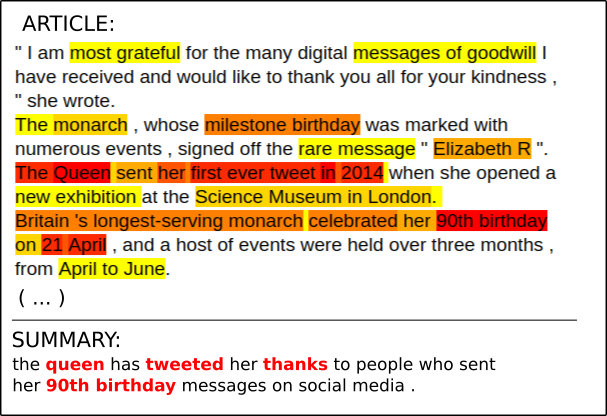
\includegraphics[width=7.6cm]{heatmap_summ_small}
%     \caption{A highlighted article and its summary which is abstracted from the first three lines of the article}
%   \label{image:heatmap_small}
% \end{figure}

\begin{figure}[h]
    \centering
    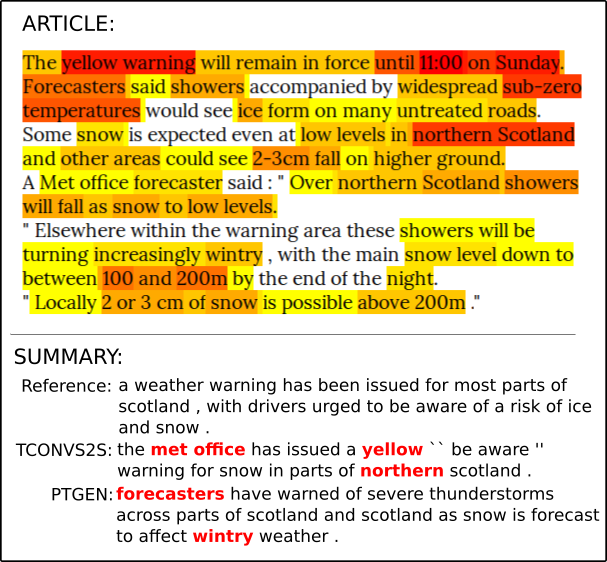
\includegraphics[width=7.6cm]{heatmap_summ_small_2}
    \caption{Highlighted article, reference summary, and summaries generated by \tconv\ and \ptgen. Words in red in the system summaries are highlighted in the article but do not appear in the reference.}
  \label{image:heatmap_small_2}
\end{figure}

\paragraph{\highres{} eliminates reference bias.}
The example presented in Figure \ref{image:heatmap_small_2} demonstrates how our highlight-based evaluation eliminates reference bias in summarization evaluation. The summaries generated by \tconv\ and \ptgen\ are able to capture the essence of the document, however, there are phrases in these summaries that do not occur in the reference summary. A reference-based evaluation would fail to give a reasonable score to these system summaries. The \highres{} however, would enable the judges to better evaluate the summaries without any reference bias.

\paragraph{Fluency vs Clarity.} Example in Table~\ref{table:fluencyclarityexample} shows disagreements between fluency and clarity scores for different summaries of the same article. From the example, we can see that the \tconv{} summary is fluent but is not easily understood in the context of `the duration of resignation', while the \ptgen{} summary has word duplication which lower the fluency and also lacking clarity due to several unclear words. 
\begin{table}[t!]
\small
\begin{tabular}{p{1.5cm}|p{3.5cm}|p{0.7cm}p{0.7cm}}
\hline
\textbf{Model}     & \textbf{Summary Text}  & \textbf{Fluency} & \textbf{Clarity} \\
\hline
\tconv{}  & dick advocaat has resigned as sunderland manager \textit{until the end of the season} .                                          & 92.80   & 44.33   \\
\ptgen{}     & sunderland have appointed \textit{former sunderland boss} dick advocaat as manager \textit{at the end of the season} to sign a \textit{new deal} . & 41.33   & 6.00    \\
\hline
\end{tabular}
\caption{%Summaries of reference, 
\tconv{} and \ptgen{} showing a disagreement between fluency and clarity scores. We italicized words that are not clear in the summaries.}
\label{table:fluencyclarityexample}
\end{table}
% how the \tconv\  and \ptgen\   summaries could be evaluated without any bias to the reference. This can be seen in our example case where some phrases in the \tconv\  and \ptgen\   summaries do not occur in the reference summary but are highlighted in the article. A reference-based 
% evaluation 
% would fail to give a justified score to those models summary. The \highres{} however, would enable the judges to better evaluate the summaries without any reference bias.

\section{Conclusion and Future Work}
In this paper we introduced the \textsc{High}light-based \textsc{R}eference-less \textsc{E}valuation \textsc{S}ummarization (\highres) framework for manual evaluation.
The proposed framework avoids reference  bias
and provides absolute instead of ranked evaluation of the systems. Our experiments show that \highres{}  lowers the variability of the judges' content assessment, while helping expose the differences between systems. We also showed that by evaluating clarity we are able to capture a different dimension of summarization quality that is not captured by the commonly used fluency. 
%while increasing the F$_1$ scores.
We believe that our highlight-based evaluation is an ideal setup of abstractive summarization for three reasons: (i) highlights can be crowd sourced effectively without expert annotations, (ii) it avoids reference bias and (iii) it is not limited by n-gram overlap.
In future work, we would like to extend our framework to other variants of summarization e.g.\  multi-document. Also, we will explore ways of automating parts of the process, e.g.\ the highlight annotation. Finally, the highlights could also be used as training signal, as it offers content saliency information at a finer level than the single reference typically used.

%\shashi{Highlights for content selection signal, during training}
\begin{footnotesize}

\section*{Acknowledgments}

Hardy would like to thank the Indonesian government that
has sponsored the first author’s studies through
the Indonesia Endowment Fund for Education
(LPDP). Shashi Narayan and Andreas Vlachos were supported by the
EU H2020 SUMMA project (grant agreement
number 688139). The latter is also supported by the EPSRC grant eNeMILP
(EP/R021643/1).


\end{footnotesize}

% The acknowledgments should go immediately before the references.  Do
% not number the acknowledgments section. Do not include this section
% when submitting your paper for review. \\
\bibliography{acl2019}
\bibliographystyle{acl_natbib}

\onecolumn
\newpage
\setcounter{section}{0}
\setcounter{figure}{0}
\setcounter{table}{0}
\section*{Supplementary Material}
\section{Highest and lowest highlight annotation agreement articles}
\begin{figure*}[h]
    \centering
    \begin{minipage}{.45\textwidth}
    \centering
    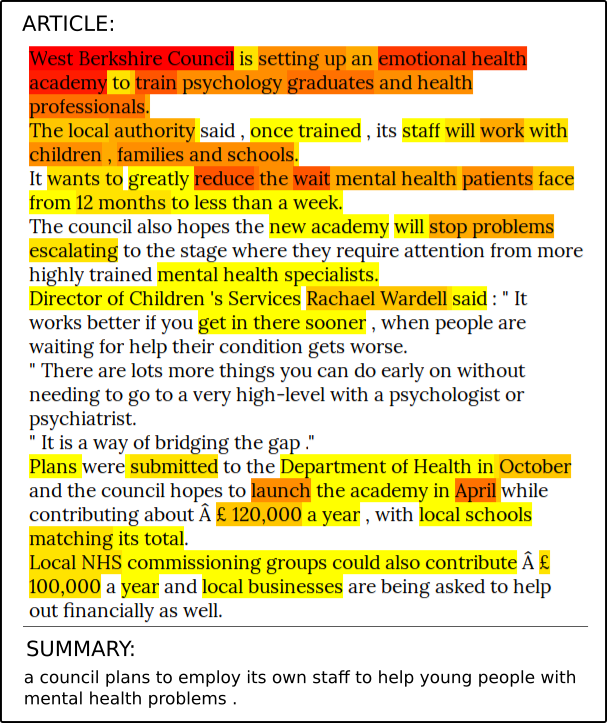
\includegraphics[height=7cm]{heatmap_best}
    \end{minipage}
    \begin{minipage}{.45\textwidth}
    \centering
    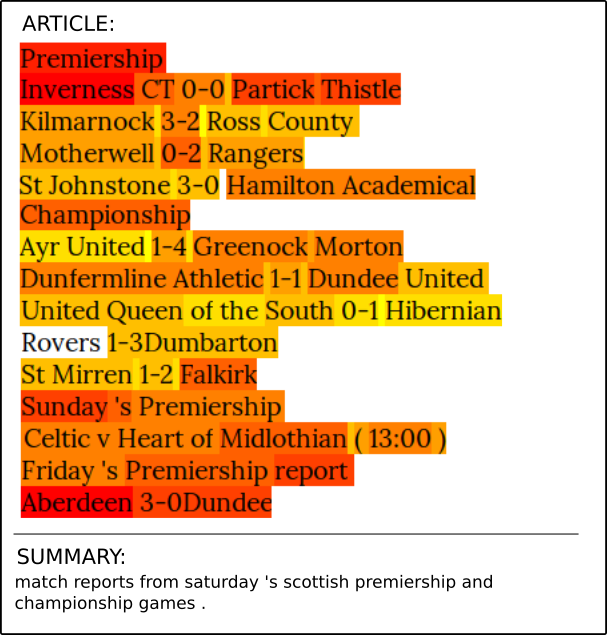
\includegraphics[height=6.5cm]{heatmap_negative}
    \end{minipage}
    \caption{Highlight annotation for the documents with the highest (left) and lowest (right) agreement. We also show their reference summaries at the bottom.}
  \label{image:heatmap_both}
\end{figure*}
\newpage
\section{Overview of Manual Evaluations}
\begin{table*}[h]
\centering
\small
\begin{tabular}{r | c | c c c c c c c | c c | c c r}

\hline
\rotatebox[origin=c]{0}{\textbf{Systems}} & 
\rotatebox[origin=l]{90}{\textbf{No Manual Eval}} & 
\rotatebox[origin=l]{90}{\textbf{Pyramid}} & \rotatebox[origin=l]{90}{\textbf{QA}} & \rotatebox[origin=l]{90}{\textbf{Correctness}} &
\rotatebox[origin=l]{90}{\textbf{Fluency}} &
\rotatebox[origin=l]{90}{\textbf{Clarity}} & \rotatebox[origin=l]{90}{\textbf{Recall}} & \rotatebox[origin=l]{90}{\textbf{Precision}} & \rotatebox[origin=l]{90}{\textbf{Absolute}} & \rotatebox[origin=l]{90}{\textbf{Relative}} & \rotatebox[origin=l]{90}{\textbf{With Reference}} & \rotatebox[origin=l]{90}{\textbf{With Document}} & \rotatebox[origin=l]{90}{\textbf{With Ref. \& Doc.}} \\
\hline
\citet{See2017}        &  $\checkmark$   &   &   &    &   &  &  &   &    &      &     &    &   \\
\citet{Lin2018}     &  $\checkmark$   &   &    &   &   &  &   &    &      &     &    &     &  \\
\citet{Cohan2018a}     &  $\checkmark$   &   &    &   &  &  &   &    &      &     &    &     &  \\
\citet{Liao2018a}      &  $\checkmark$   &   &    &   &  &  &   &    &      &     &    &    &  \\
\citet{Kedzie2018}     &  $\checkmark$   &   &    &   &  &  &   &    &      &     &    &    & \\
\citet{Amplayo2018a}   &  $\checkmark$   &   &    &   &  &  &   &    &      &    &     &    & \\
\citet{Jadhav2018}    &  $\checkmark$   &   &    &   &  &  &   &    &      &    &     &   &  \\
\citet{li2018guiding}        &  $\checkmark$   &   &    &   &  &  &   &      &     &    &     &    & \\
\citet{Pasunuru2018a}  &  $\checkmark$   &   &    &   &  &  & &      &     &    &     &    & \\
\citet{Cao2018a}       &  $\checkmark$   &   &    &   &  &    &    &      &     &    &     &    & \\
\citet{Sakaue2018a}    &  $\checkmark$   &   &    &   &   &   &    &      &     &    &     &   & \\
\citet{Celikyilmaz2018}      &    &  &  &    &  &  &  $\checkmark$ &  $\checkmark$    &  $\checkmark$   &  $\checkmark$     &  $\checkmark$    &  $\checkmark$   & \\
\citet{Chen2018a}     &   &   &  & $\checkmark$   & & &  $\checkmark$ &  $\checkmark$    &    &  $\checkmark$     &     &    &  $\checkmark$   \\

\citet{Guo2018a}     &      &   &  &   &  $\checkmark$  & &  &  $\checkmark$    &    &  $\checkmark$     &     &    &  $\checkmark$  \\
\citet{Hardy2018}    &     &   &  &   & $\checkmark$  & &   &     & $\checkmark$  &      &     &    &   \\
\citet{Hsu2018}      &      &  &  &    &  $\checkmark$  & &  $\checkmark$ &  $\checkmark$    &  $\checkmark$   &      &     &  $\checkmark$   &  \\
\citet{Krishna2018a}    &      &   &  &   &  &  &  $\checkmark$ &     &    &  $\checkmark$     &     &  $\checkmark$   &    \\
\citet{Kryscinski2018}    &    &   &  &   &  $\checkmark$ & &  $\checkmark$ & &  $\checkmark$   &      &  & $\checkmark$ &   \\
\citet{Li2018a}     &       &   &   & $\checkmark$ &  &  &   &     &  $\checkmark$   &      &     &     &    \\
\citet{narayan-sidenet18}    &     & &   &    &  $\checkmark$ & &  &     &    & $\checkmark$ &  &  $\checkmark$   &    \\
\citet{narayan18xsum}       &      &   &  $\checkmark$ &    &  $\checkmark$ &  &  $\checkmark$ &     &  $\checkmark$  &  $\checkmark$     &   $\checkmark$  &  $\checkmark$   &   \\
\citet{Narayan2018}     &     &   & $\checkmark$ &   &  $\checkmark$  & &  $\checkmark$ &     &  $\checkmark$  &  $\checkmark$   &  $\checkmark$   &  $\checkmark$  &   \\
\citet{Peyrard2018a}    &    &   &  &   &  &  &  $\checkmark$ &  $\checkmark$    &  $\checkmark$   &      &  $\checkmark$    &    &   \\
\citet{ShafieiBavani2018}   &      &  $\checkmark$ &  &    &  &  &  &     &    &      &     &    &  \\
\citet{Song2018}      &    &   &  & $\checkmark$   &  $\checkmark$ &  &  $\checkmark$ &     &  $\checkmark$   &      &     &  $\checkmark$   & \\
\citet{Yang2017b}      &    &  &  &    &  &  &  $\checkmark$ &     &    &  $\checkmark$     &  $\checkmark$    &    & \\
\highres\ (ours)    &   &   &  &   & $\checkmark$ & $\checkmark$ & $\checkmark$  &  $\checkmark$   & $\checkmark$  &      &     &  $\checkmark$  &   \\
\hline
\end{tabular}
\caption{Overview of manual evaluations conducted in recent summarization systems. We categorize them in four dimensions: the first columns presents papers that do not report on human evaluation; the second column identifies matrices used for evaluating content (``\textit{Pyramid}'', ``\textit{QA}'', ``\textit{Correctness}'', ``\textit{Recall}'' and ``\textit{Precision}'') and quality (``\textit{Clarity}'', ``\textit{Fluency}'') of summaries; the third column focuses if the system ranking reported by humans on content evaluation were ``\textit{Absolute}'' or ``\textit{Relative}''; and finally, the fourth column evaluates if summaries were evaluated against the input document (``\textit{With Document}''), the reference summary (``\textit{With Reference}'') or both (``\textit{With Ref. \& Doc.}'').}
\end{table*}
\newpage
\section{HighRES User Interface Screenshots}
\begin{figure}[h]
    \centering
    \fbox{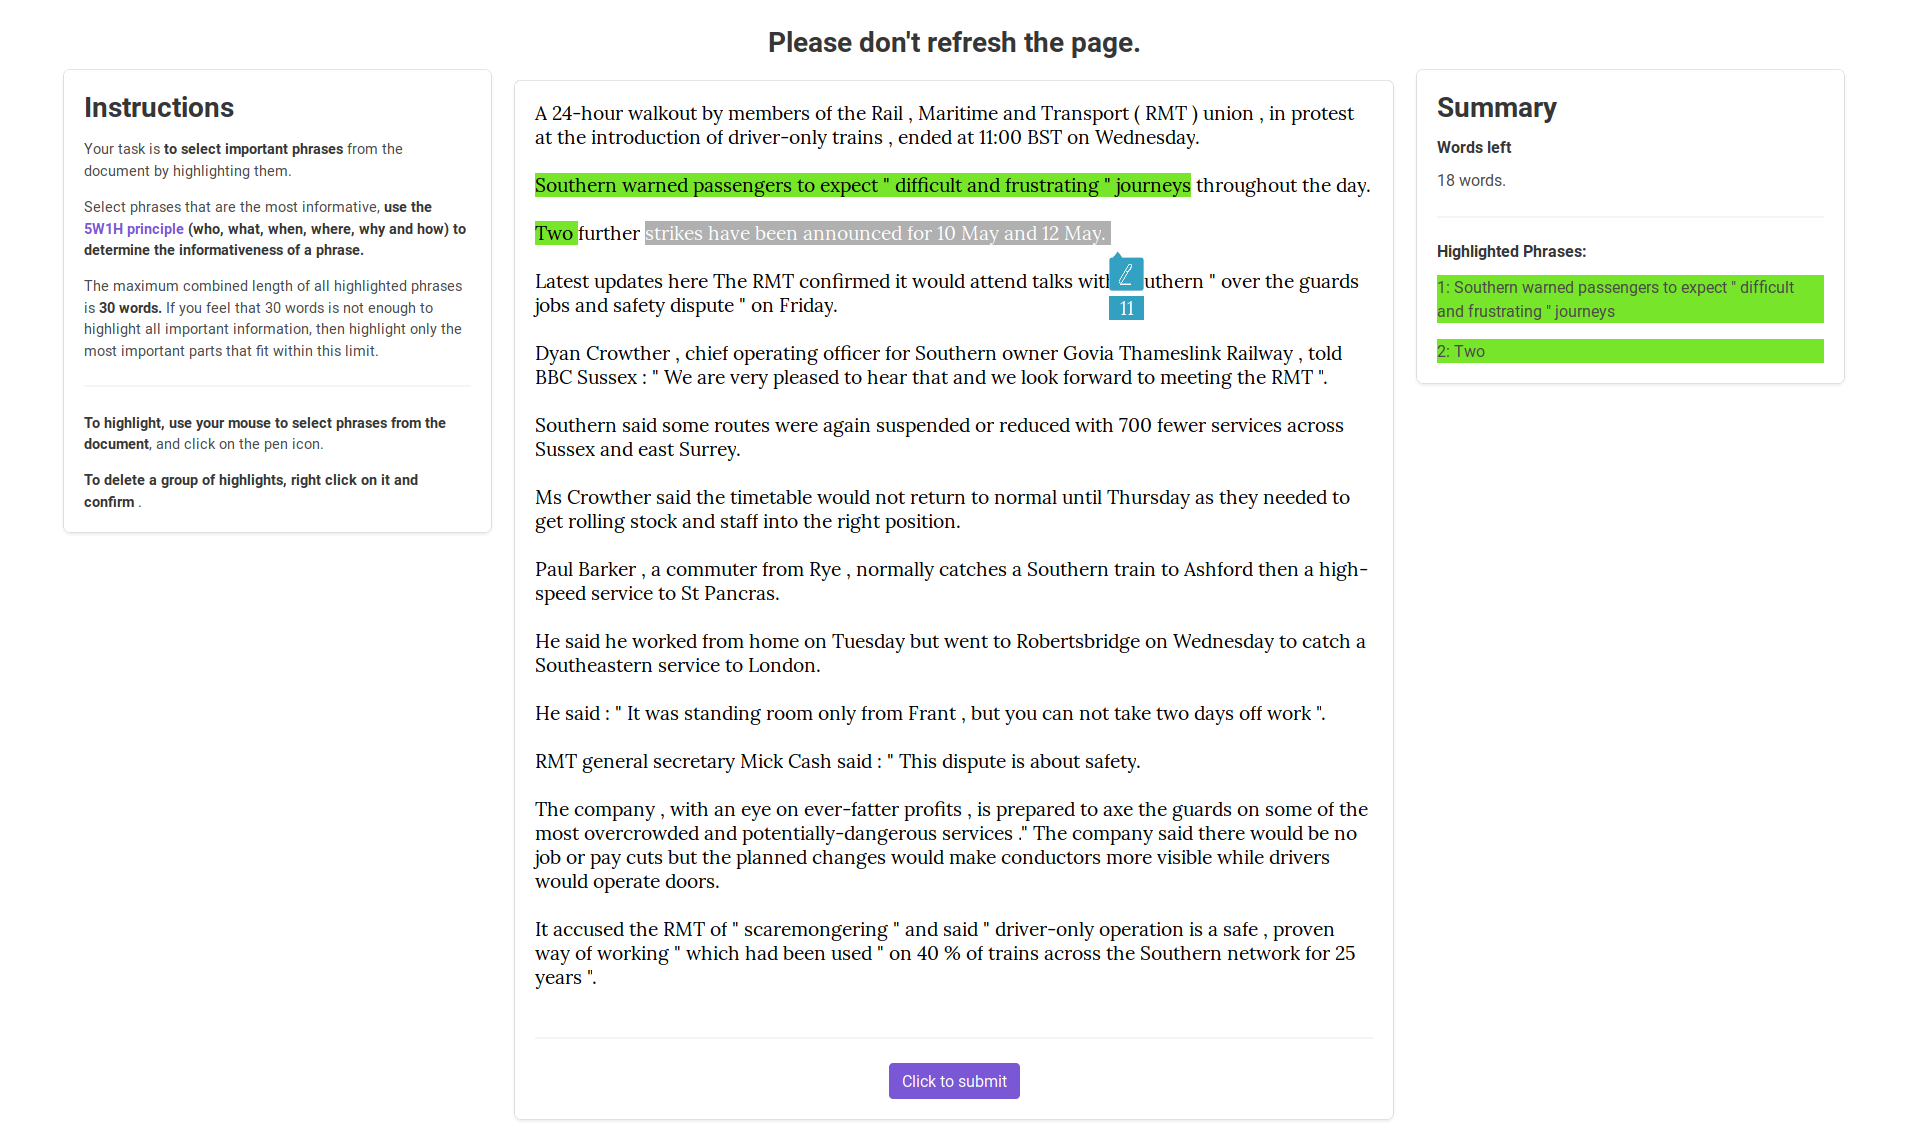
\includegraphics[width=17cm]{annotation}}
    \caption{The UI for highlight annotation. Judges are given an article and asked to highlight words or phrases that are important in the article.}
\end{figure}
\begin{figure}[h]
    \centering
    \fbox{
\includegraphics[width=17cm]{annotation_sanity}}
    \caption{The sanity checking question at the end of the annotation task.}
\end{figure}

\begin{figure}[h]
    \centering
    \fbox{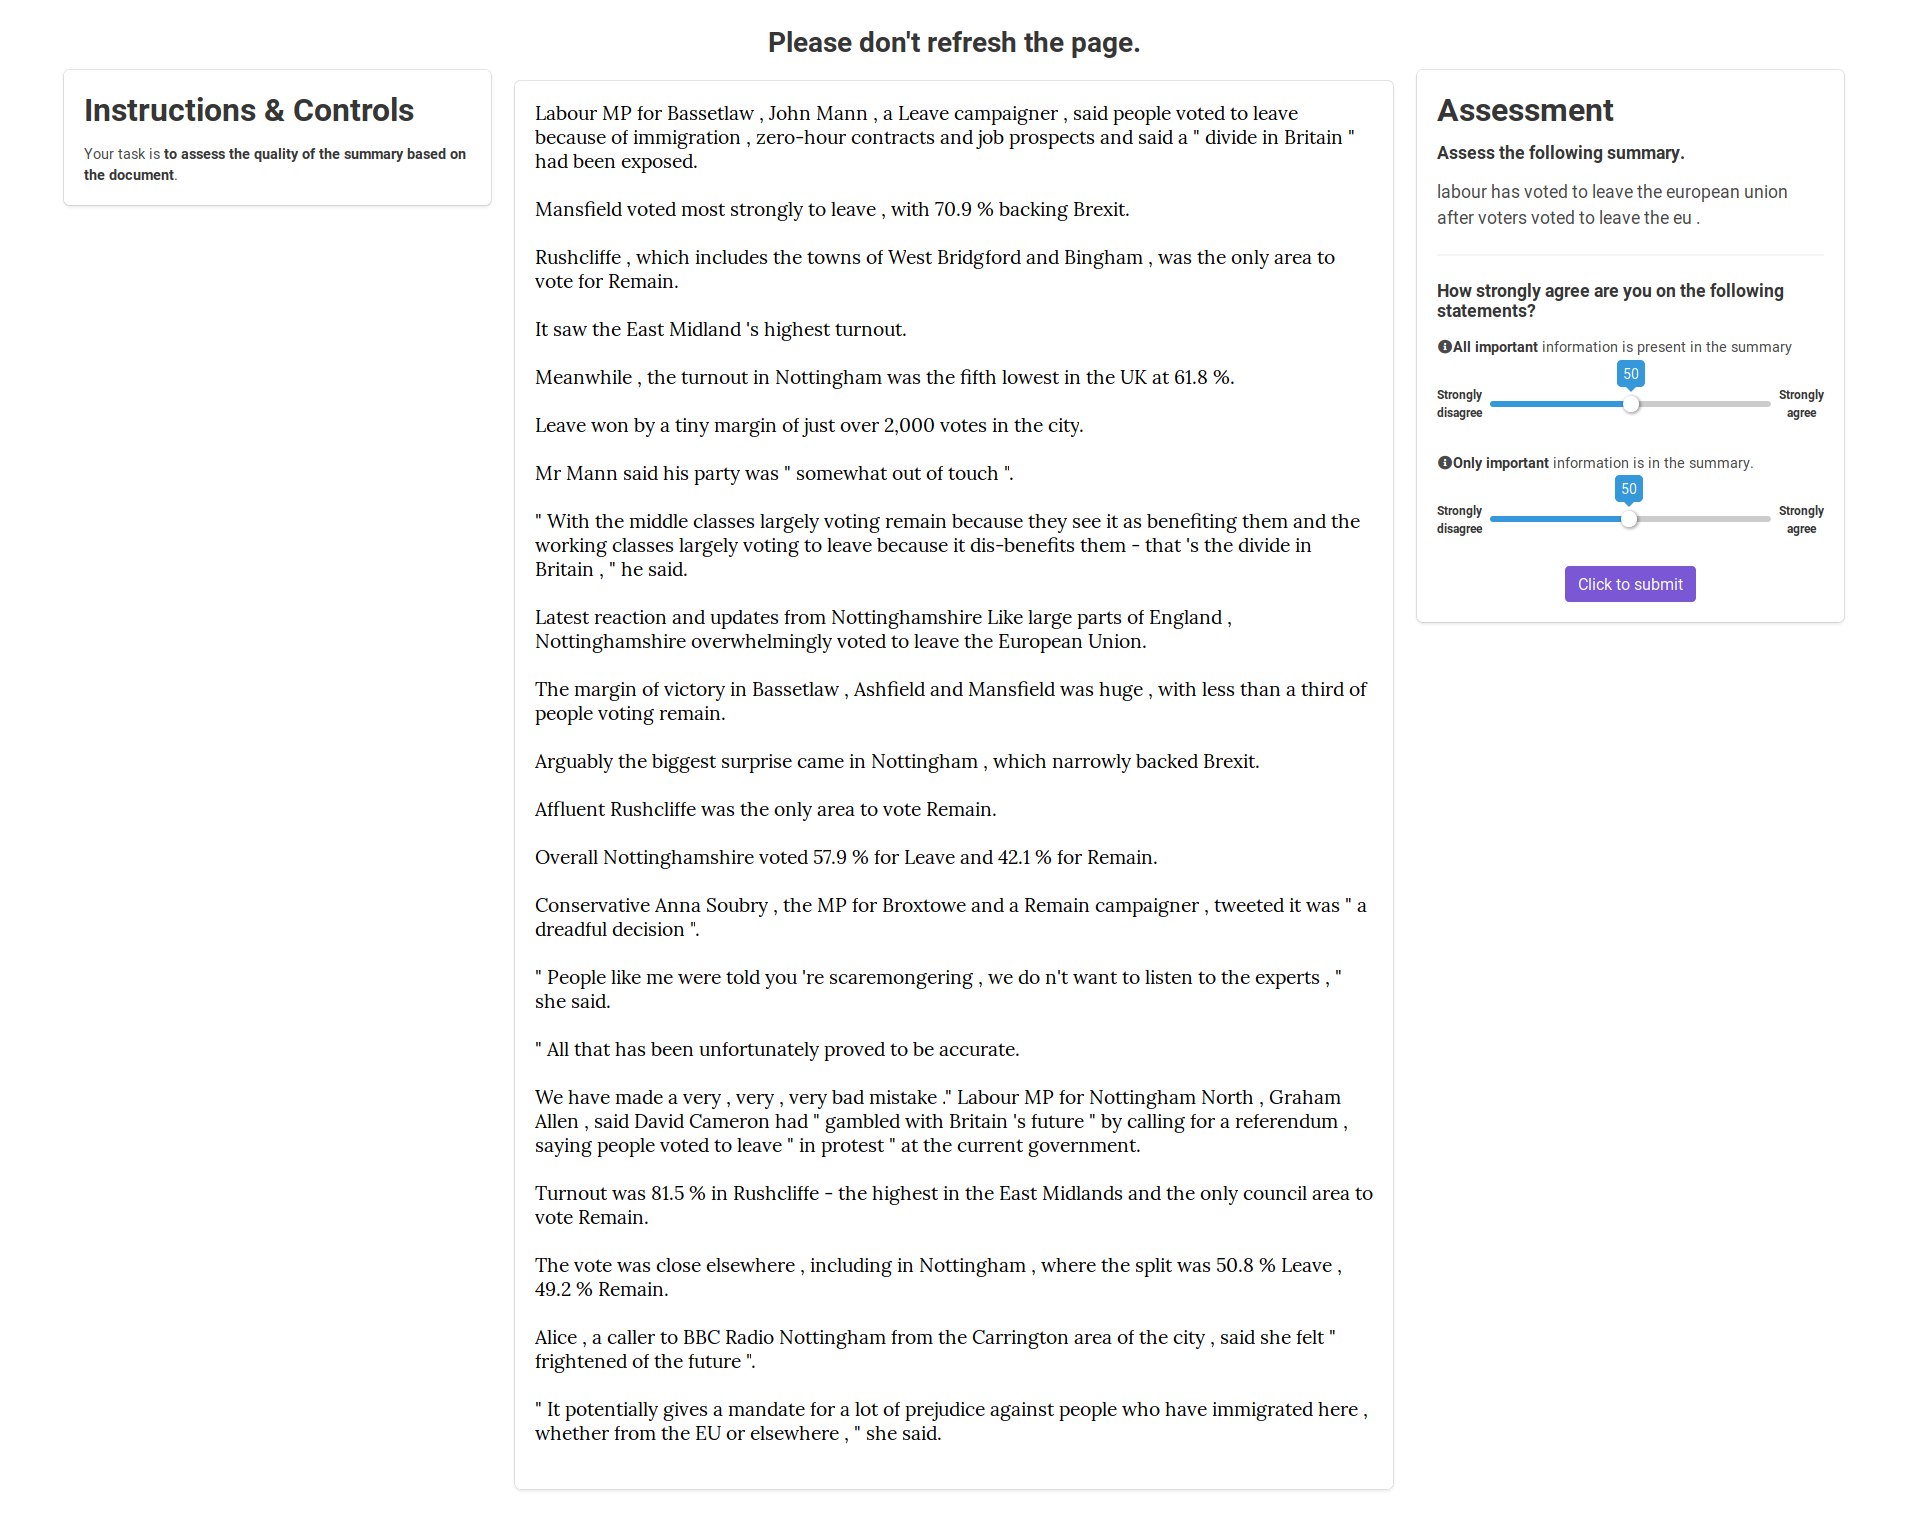
\includegraphics[width=17cm]{non_highlight_evaluation}}
    \caption{The UI for content evaluation without highlight. At the right of the page judges give the recall and precision assessment by sliding the scroller from 1 to 100 based on the given summary quality.}
    \label{fig:my_label}
\end{figure}
\begin{figure}[h]
    \centering
    \fbox{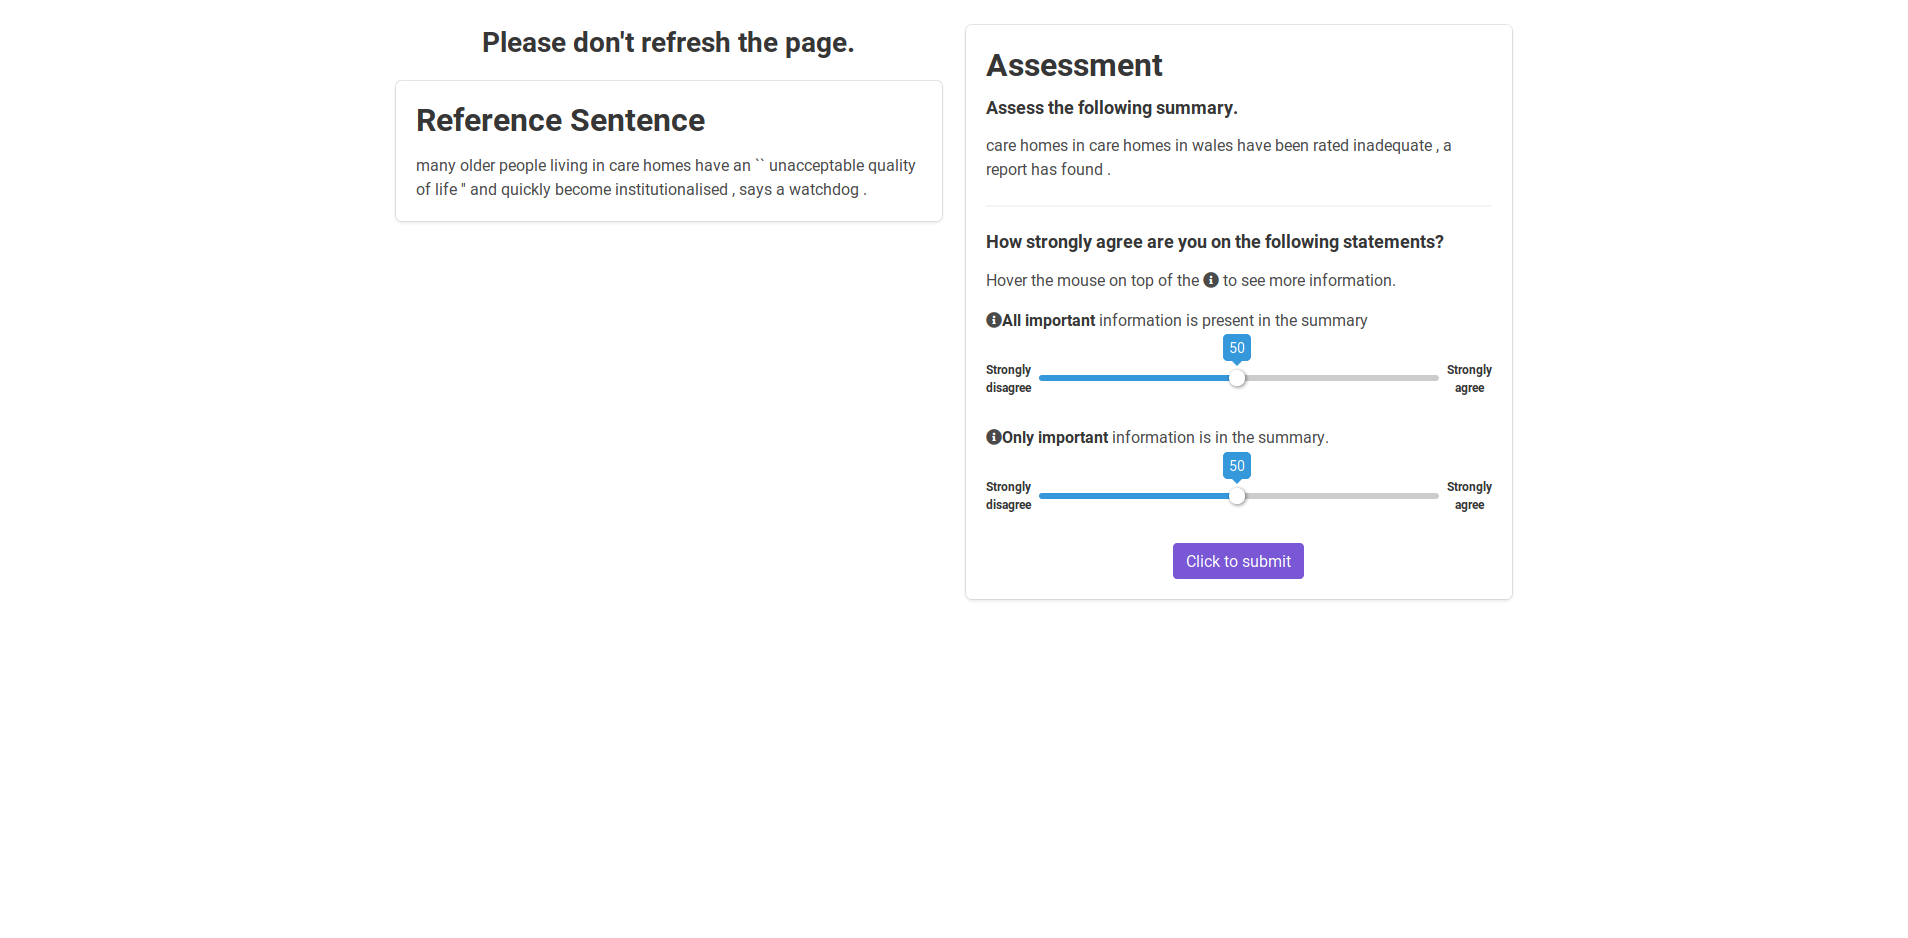
\includegraphics[width=17cm]{ref_evaluation}}
    \caption{The UI for content evaluation using reference summary as comparison. At the right of the page judges give the recall and precision assessment by sliding the scroller from 1 to 100 based on the given summary quality.}
\end{figure}
\newpage
\begin{figure}[h]
    \centering
    \fbox{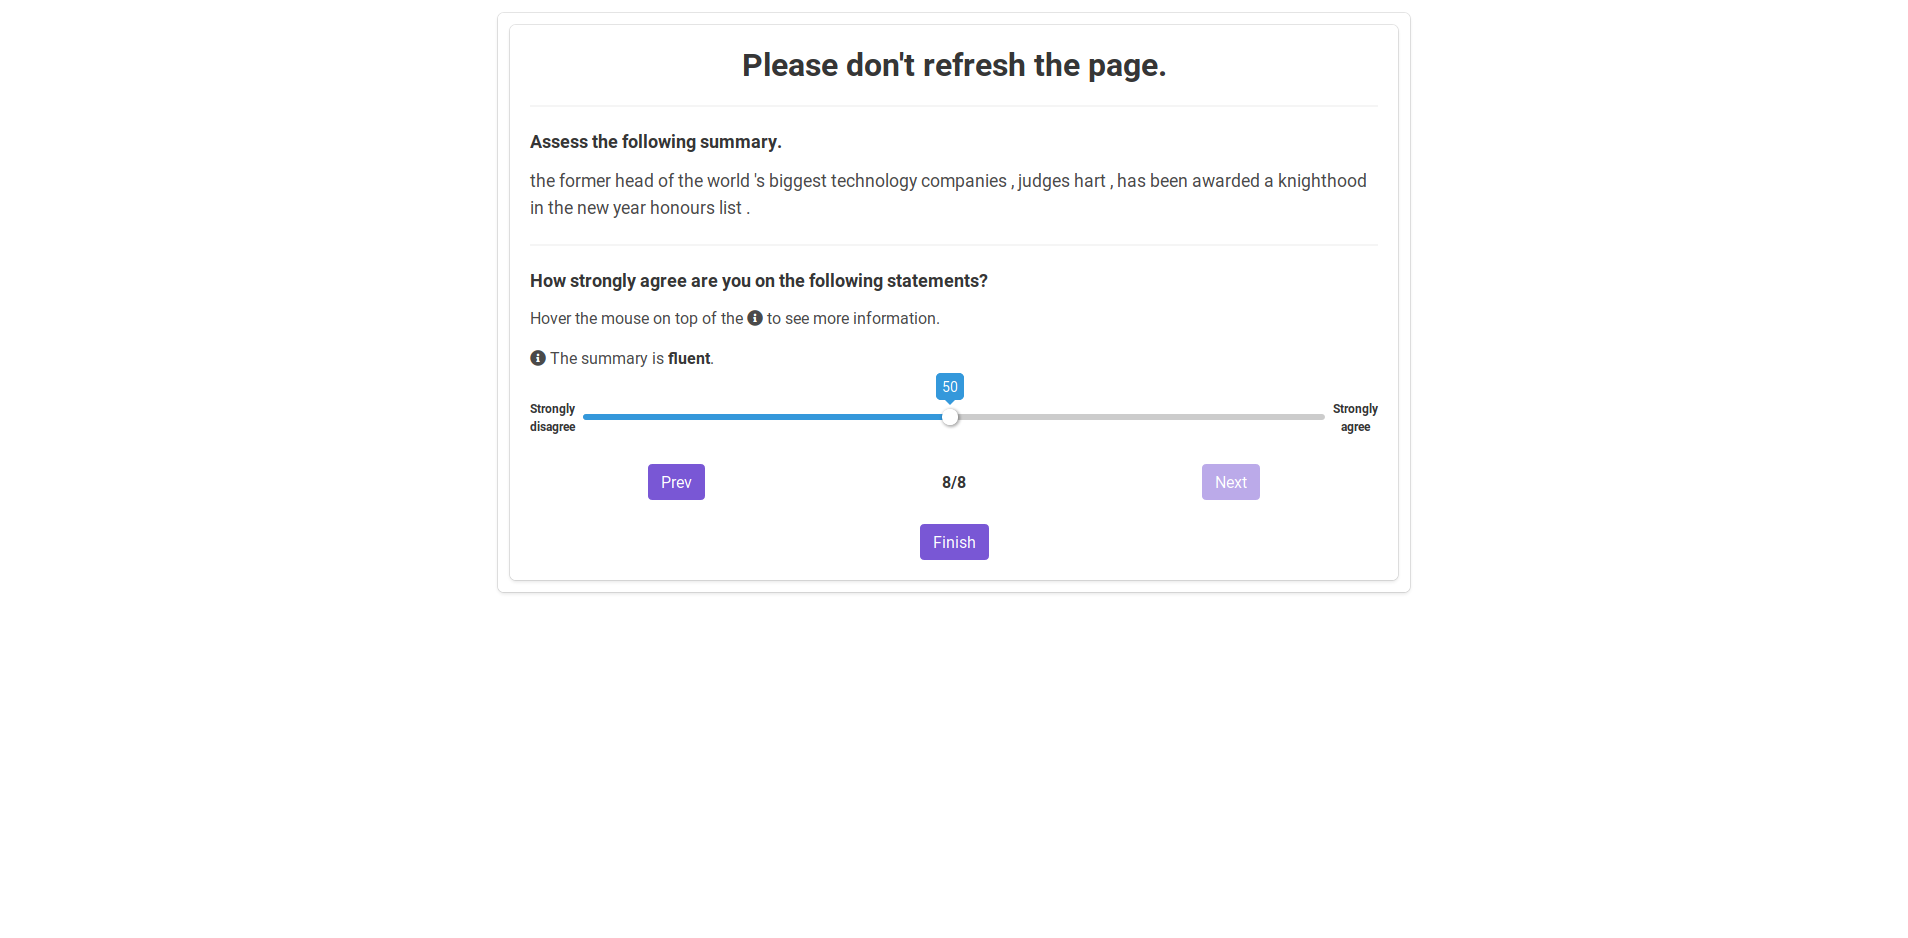
\includegraphics[width=17cm]{fluency}}
    \caption{The UI for fluency evaluation. Judges are given a number of summaries which can be switched by pressing the `Prev' or `Next' button. To give assessment, there is a scroller from 1 to 100.}
\end{figure}
\begin{figure}[h]
    \centering
    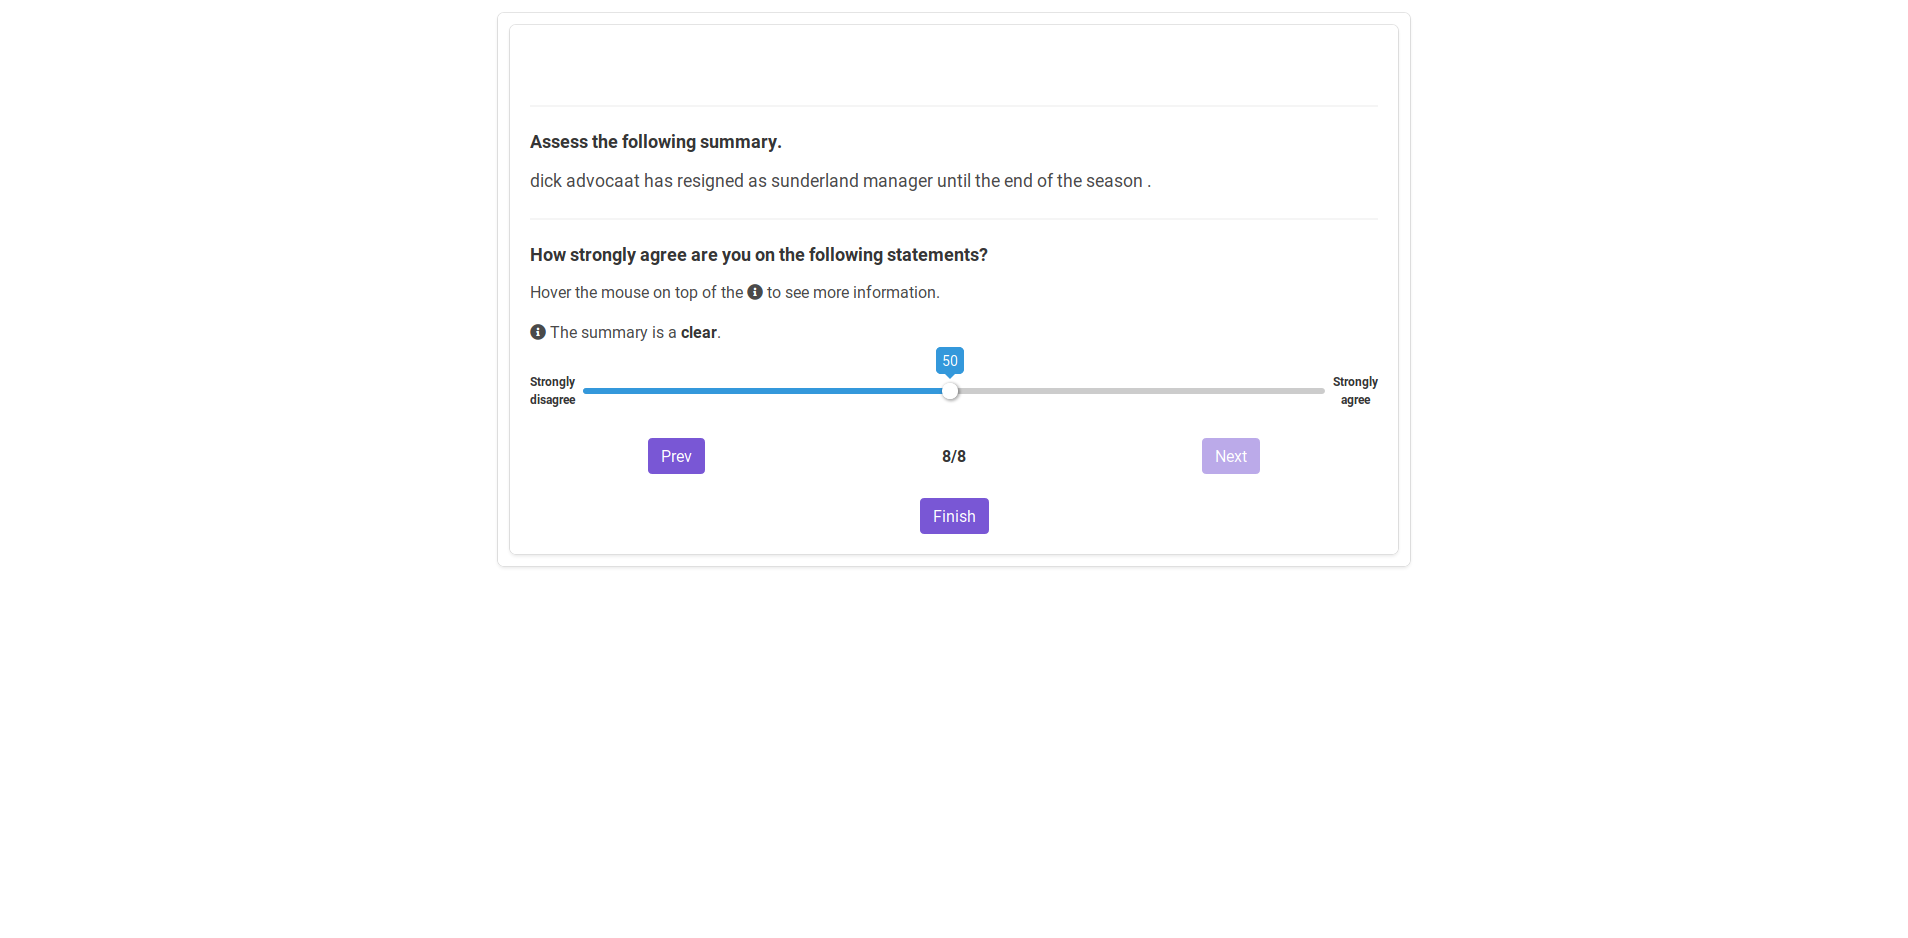
\includegraphics[width=17cm]{clarity}
    \caption{The UI for clarity evaluation. Judges are given a number of summaries which can be switched by pressing the `Prev' or `Next' button. To give assessment, there is a scroller from 1 to 100.}
\end{figure}
\end{document}

highlights for content selection signal, training

-- negative example

-- bib fix